\documentclass[compress]{beamer}
\usepackage{ifthen,verbatim,ulem}

\newcommand{\isnote}{}
\xdefinecolor{lightyellow}{rgb}{1.,1.,0.25}
\xdefinecolor{darkblue}{rgb}{0.1,0.1,0.7}

%% Uncomment this to get annotations
%% \def\notes{\addtocounter{page}{-1}
%%            \renewcommand{\isnote}{*}
%% 	   \beamertemplateshadingbackground{lightyellow}{white}
%%            \begin{frame}
%%            \frametitle{Notes for the previous page (page \insertpagenumber)}
%%            \itemize}
%% \def\endnotes{\enditemize
%% 	      \end{frame}
%%               \beamertemplateshadingbackground{white}{white}
%%               \renewcommand{\isnote}{}}

%% Uncomment this to not get annotations
\def\notes{\comment}
\def\endnotes{\endcomment}

\setbeamertemplate{navigation symbols}{}
\setbeamertemplate{headline}{\mbox{ } \hfill
\begin{minipage}{5.5 cm}
\vspace{-0.75 cm} \small
\end{minipage} \hfill
\begin{minipage}{4.5 cm}
\vspace{-0.75 cm} \small
\begin{flushright}
\ifthenelse{\equal{\insertpagenumber}{1}}{}{Jim Pivarski \hspace{0.2 cm} \insertpagenumber\isnote/\pageref{numpages}}
\end{flushright}
\end{minipage}\mbox{\hspace{0.2 cm}}\includegraphics[height=1 cm]{../cmslogo} \hspace{0.1 cm} \includegraphics[height=1 cm]{../tamulogo} \hspace{0.01 cm} \vspace{-1.05 cm}}

\begin{document}
\begin{frame}
\vfill
\begin{center}
\textcolor{darkblue}{\Large Apparent Non-Rigid Body Distortions of the DTs \\ \vspace{0.2 cm} from Tracks}

\vfill
\begin{columns}
\column{0.3\linewidth}
\begin{center}
\large
\textcolor{darkblue}{Jim Pivarski}

\vspace{0.2 cm}
Alexei Safonov
\end{center}
\end{columns}

\begin{columns}
\column{0.3\linewidth}
\begin{center}
\scriptsize
{\it Texas A\&M University}
\end{center}
\end{columns}

\vfill
 5 February, 2009

\end{center}
\end{frame}

%% \begin{notes}
%% \item This is the annotated version of my talk.
%% \item If you want the version that I am presenting, download the one
%% labeled ``slides'' on Indico (or just ignore these yellow pages).
%% \item The annotated version is provided for extra detail and a written
%% record of comments that I intend to make orally.
%% \item Yellow notes refer to the content on the {\it previous} page.
%% \item All other slides are identical for the two versions.
%% \end{notes}

\small

\begin{frame}
\frametitle{Overview}

\begin{itemize}
\item Last week, I pointed out that DT chambers appear to be ``stretched''
  in my presentation of alignment results, but we didn't have time for the details

\item In terms of residuals, it's as important as the
  alignment
\begin{itemize}
\item unbiased residuals on the $+x$ and $-x$ edges of the chambers
  differ by 5~mm
\item no translation or (reasonable) rotation of the chambers can
  account for that
\end{itemize}

\item In this talk, I'll show where the conclusion comes from, and
  what kinds of distortions we're talking about when we refer to ``stretching''

\item For completeness, one of these is the relative $\Delta R$ of
  superlayers, not what anyone would call ``stretching'' (though
  non-rigid from a chamber point of view)

\item This talk is largely the same as the ``Epilogue'' of last week's talk
\end{itemize}
\end{frame}

\begin{frame}
\frametitle{The clue (\only<1>{1}\only<2>{2}\only<3>{3}/3)}

\only<1>{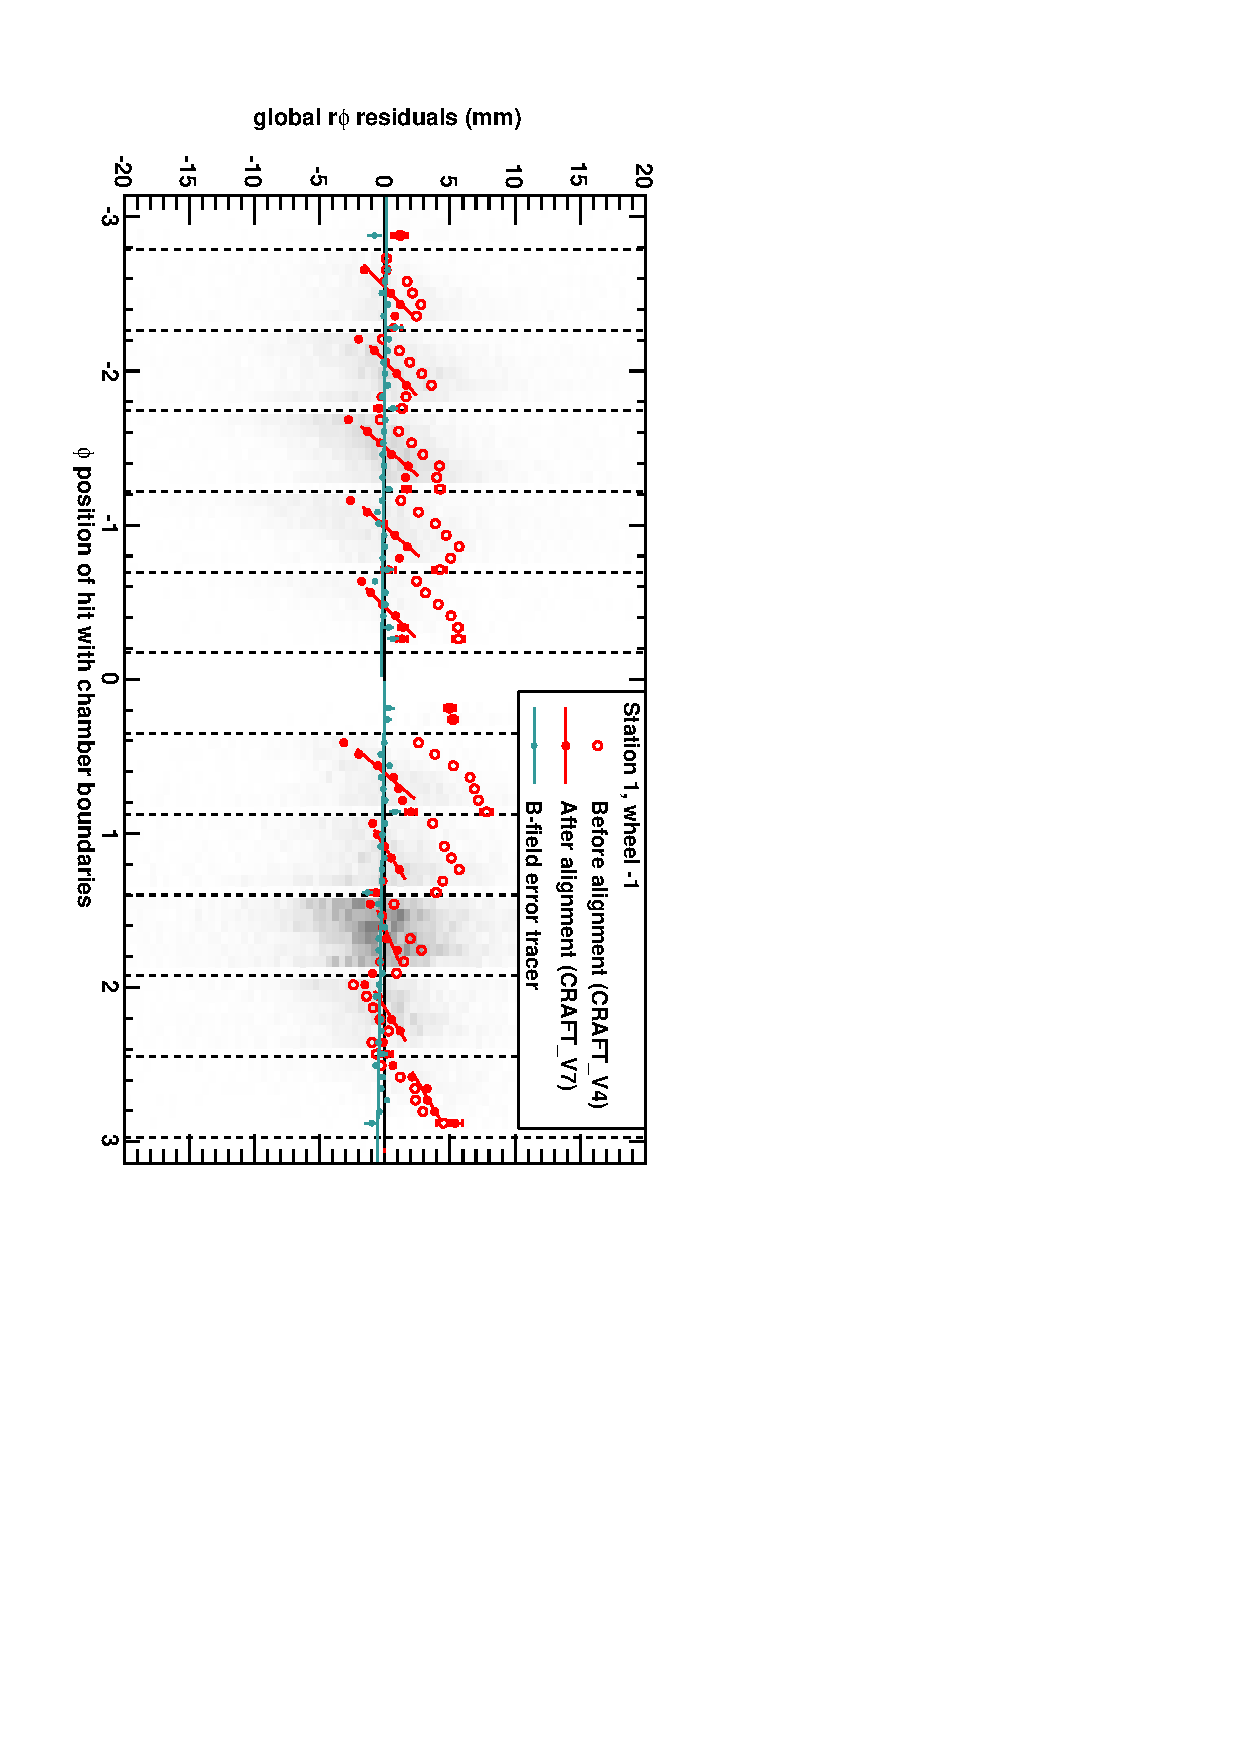
\includegraphics[height=\linewidth, angle=90]{DTrphiVsPhi_st1_whB.pdf}}
\only<2>{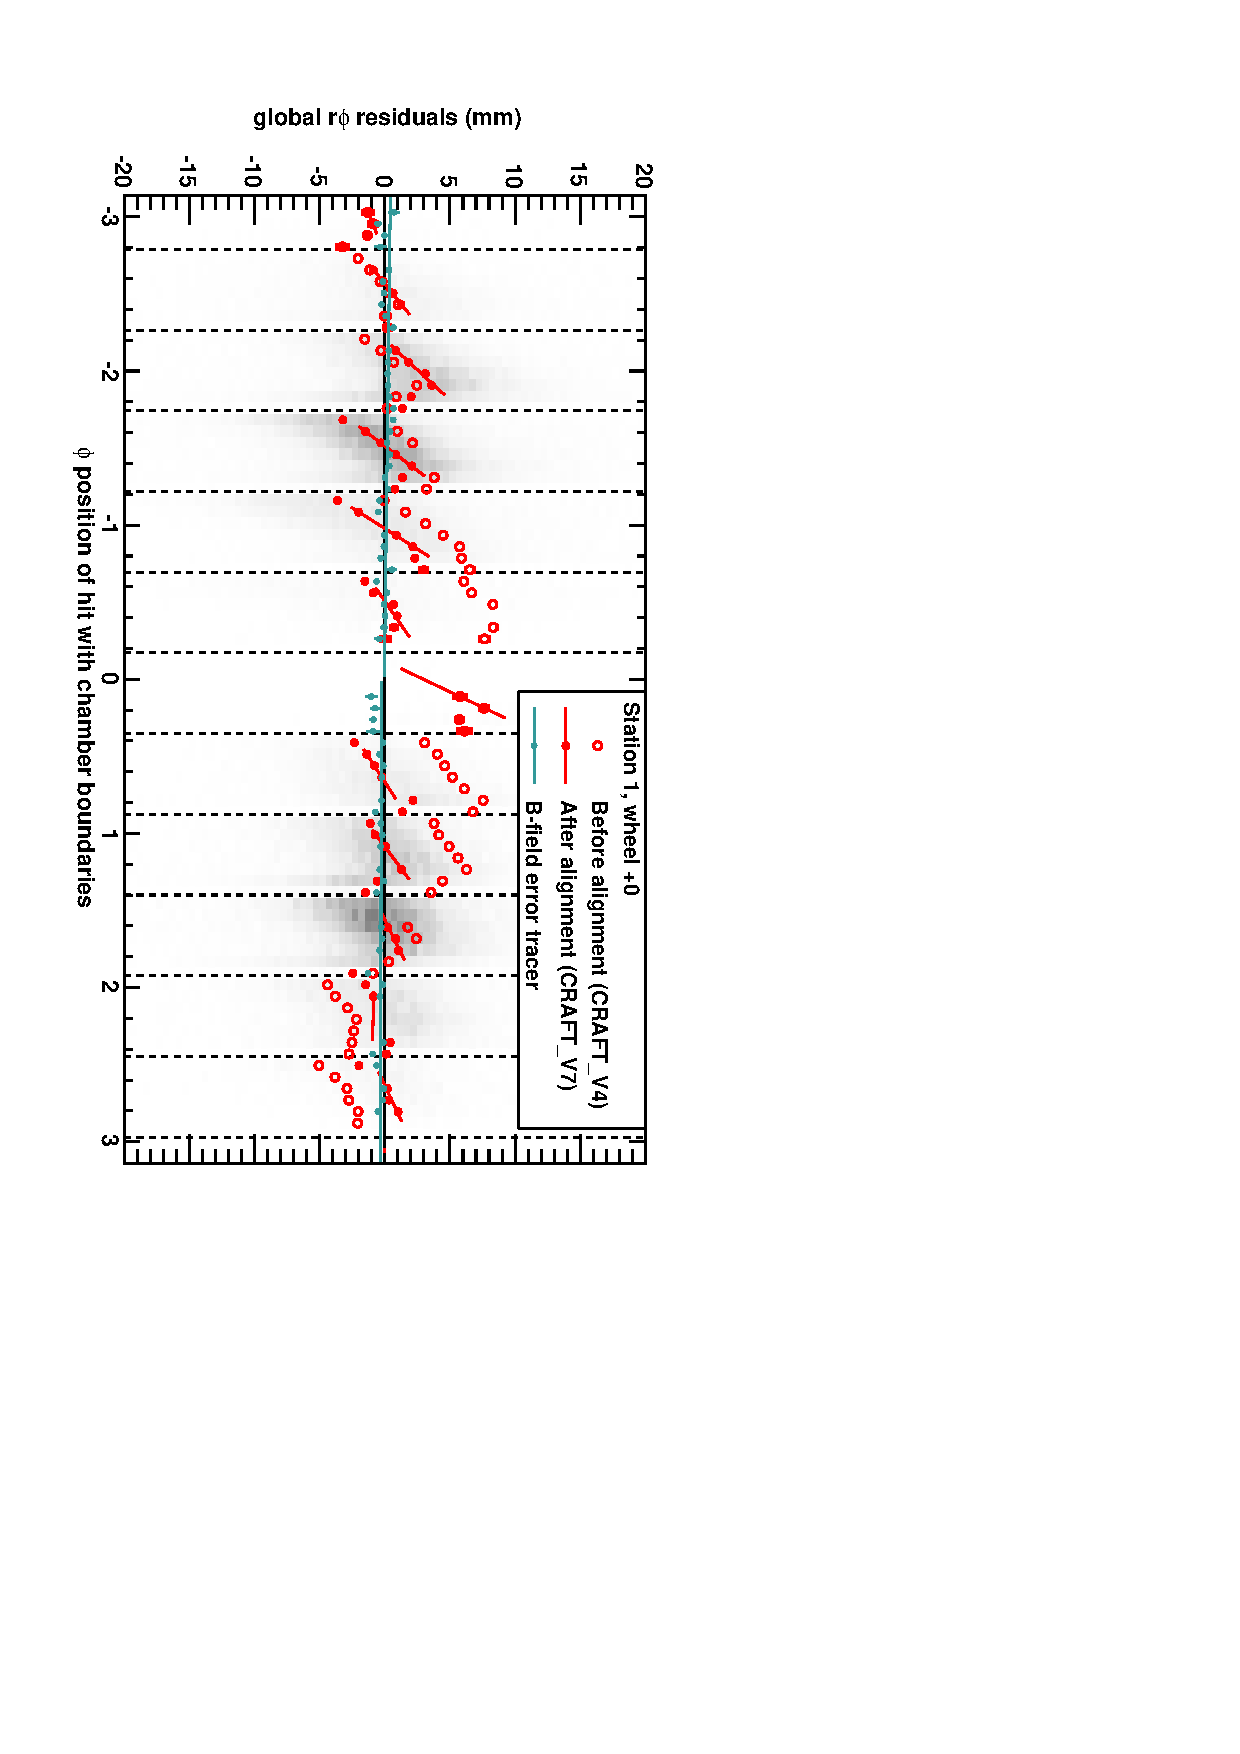
\includegraphics[height=\linewidth, angle=90]{DTrphiVsPhi_st1_whC.pdf}}
\only<3>{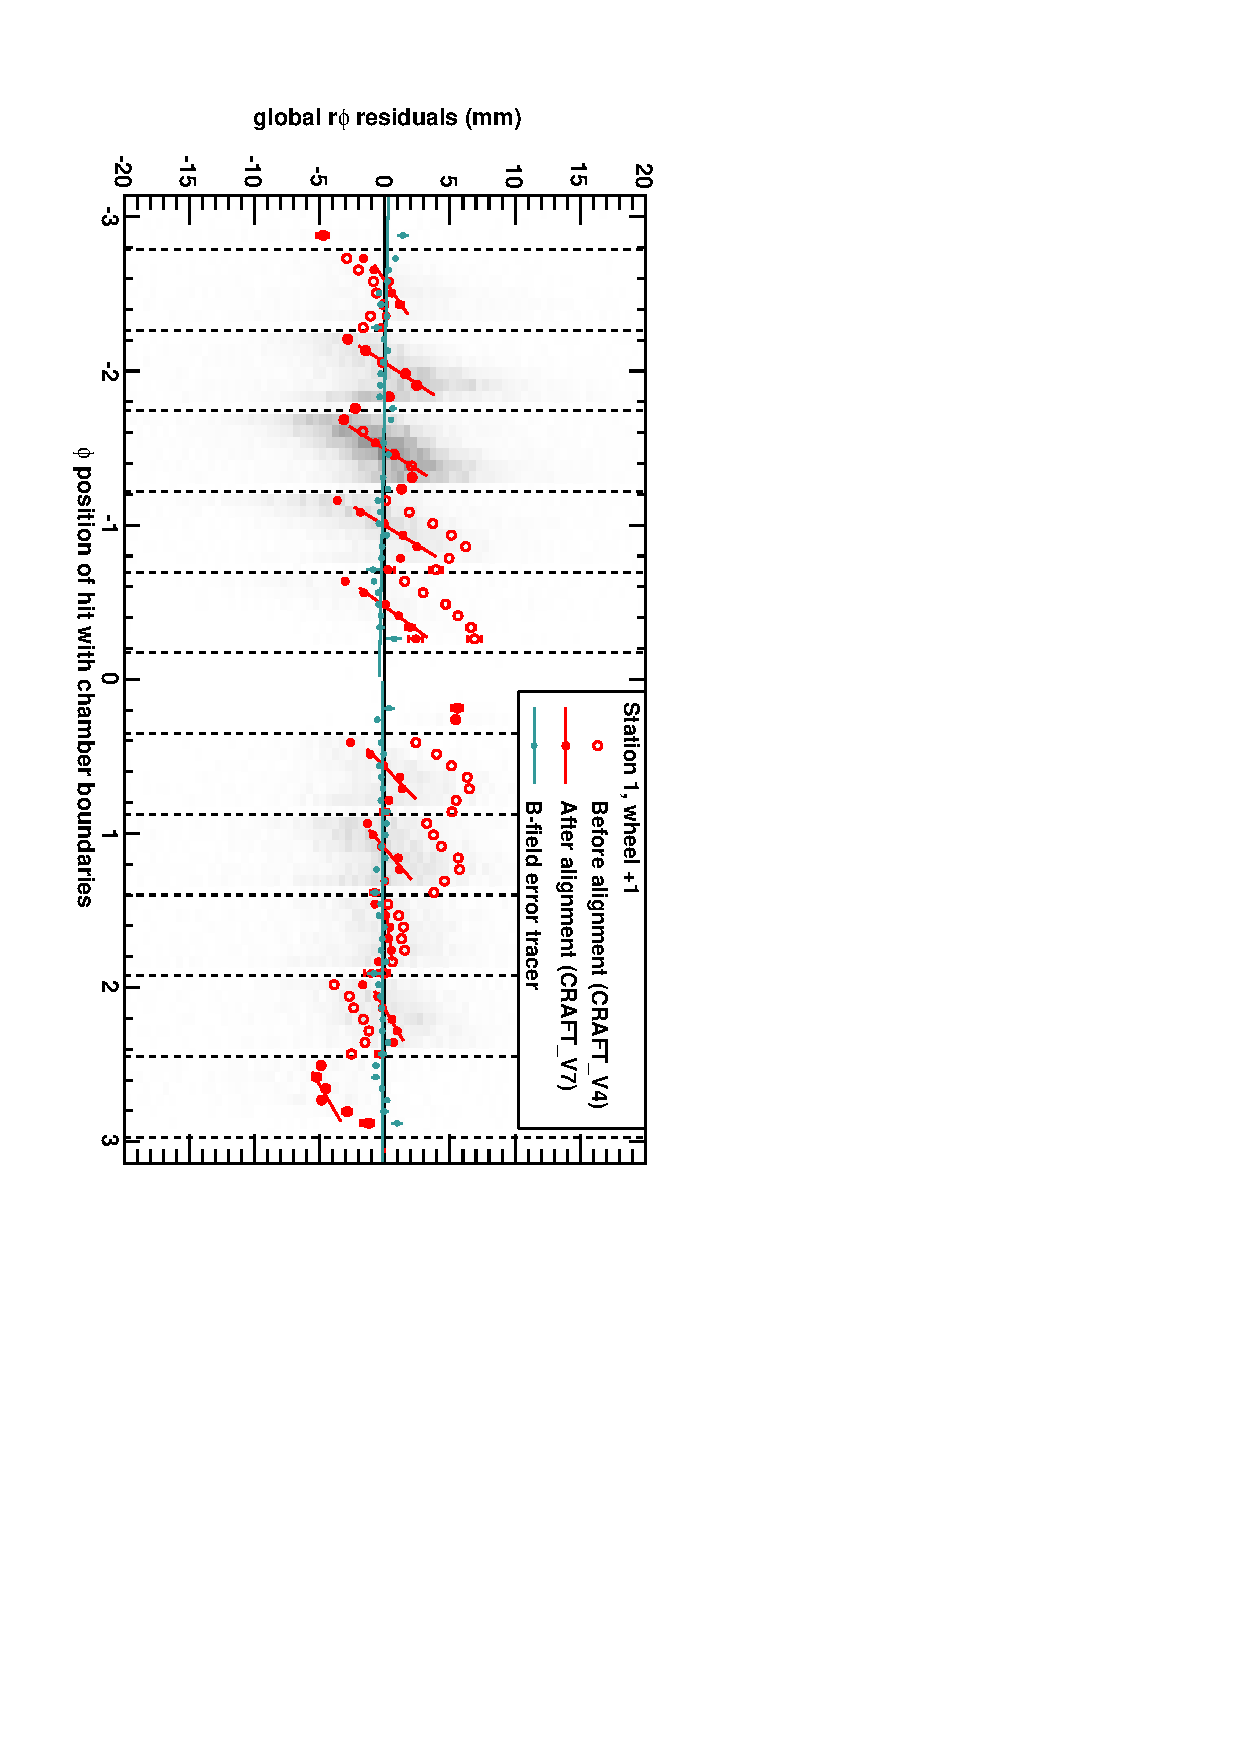
\includegraphics[height=\linewidth, angle=90]{DTrphiVsPhi_st1_whD.pdf}}

\vspace{-0.5 cm}
\only<1>{\begin{itemize}
\item Linear trends in unbiased $r\phi$ residual vs.\ $\phi$ inside each chamber
\item Unaffected by local $x$ alignment (as expected)
\item Curious thing: they all seem to have (more or less) the same slope
\end{itemize}}
\only<2>{\begin{itemize}
\item What if it's a linear bias in the distribution from the track source, partly absorbed by the alignment?
\begin{itemize}
\item impossible: $\phi$ must have periodic boundary conditions
\item if we realigned chambers to make a continuous line, it could not match at $\pm\pi$ (it would fail a ``closure condition'')
\end{itemize}
\end{itemize}}
\only<3>{\begin{itemize}
\item So it's a real effect related to the chambers, not the track source
\begin{itemize}
\item not fixing it would smear chamber resolution by 5~mm!
\end{itemize}
\item What rigid body misalignments can cause it?
\begin{itemize}
\item $\phi_y$ (rotation around axis parallel to the beamline)
\item $\Delta R$ (radial displacements)
\end{itemize}
\end{itemize}}
%% \hspace{-0.83 cm} \textcolor{darkblue}{\Large Outline2}
\end{frame}

\begin{frame}
\frametitle{Full disclosure (\only<1>{1}\only<2>{2}\only<3>{3}\only<4>{4}\only<5>{5}\only<6>{6}\only<7>{7}\only<8>{8}\only<9>{9}/9)}

\only<1>{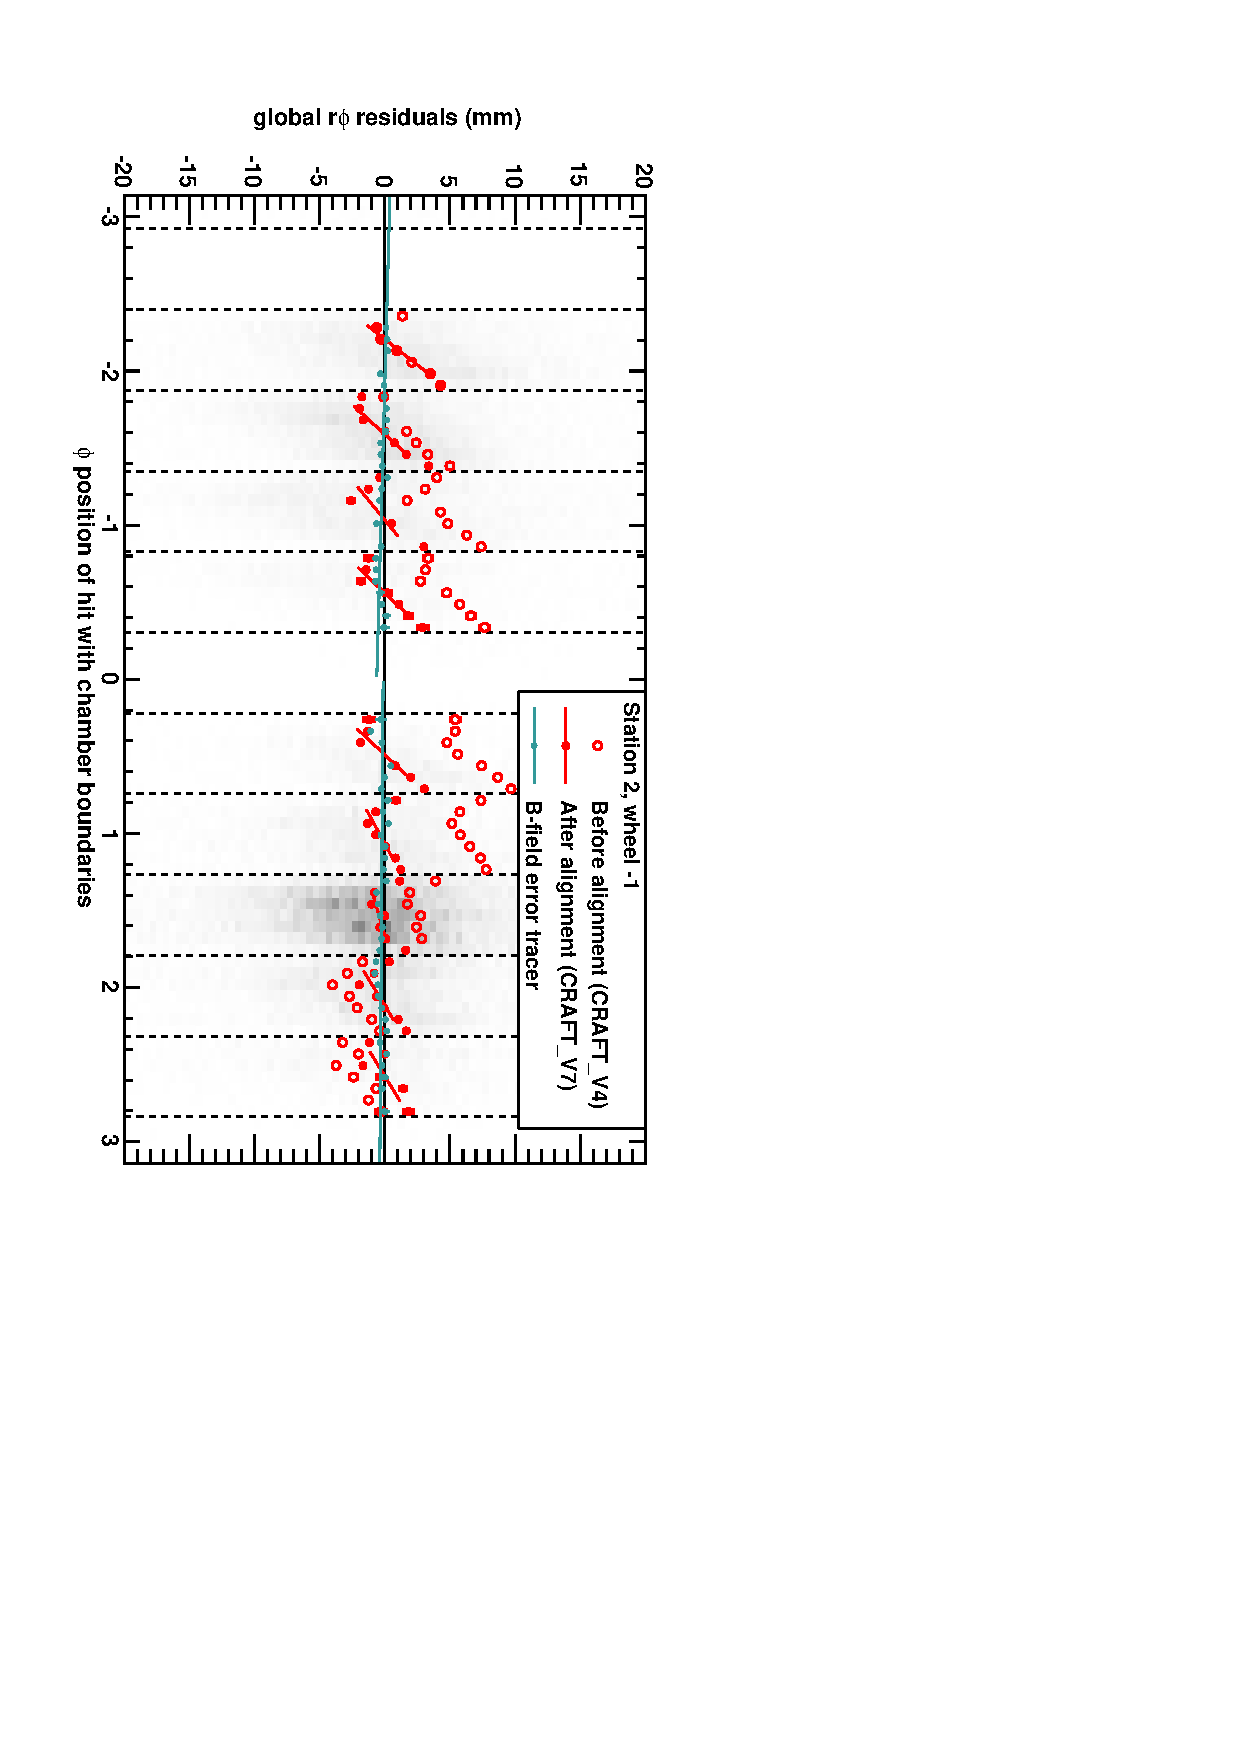
\includegraphics[height=\linewidth, angle=90]{DTrphiVsPhi_st2_whB.pdf}}\only<2>{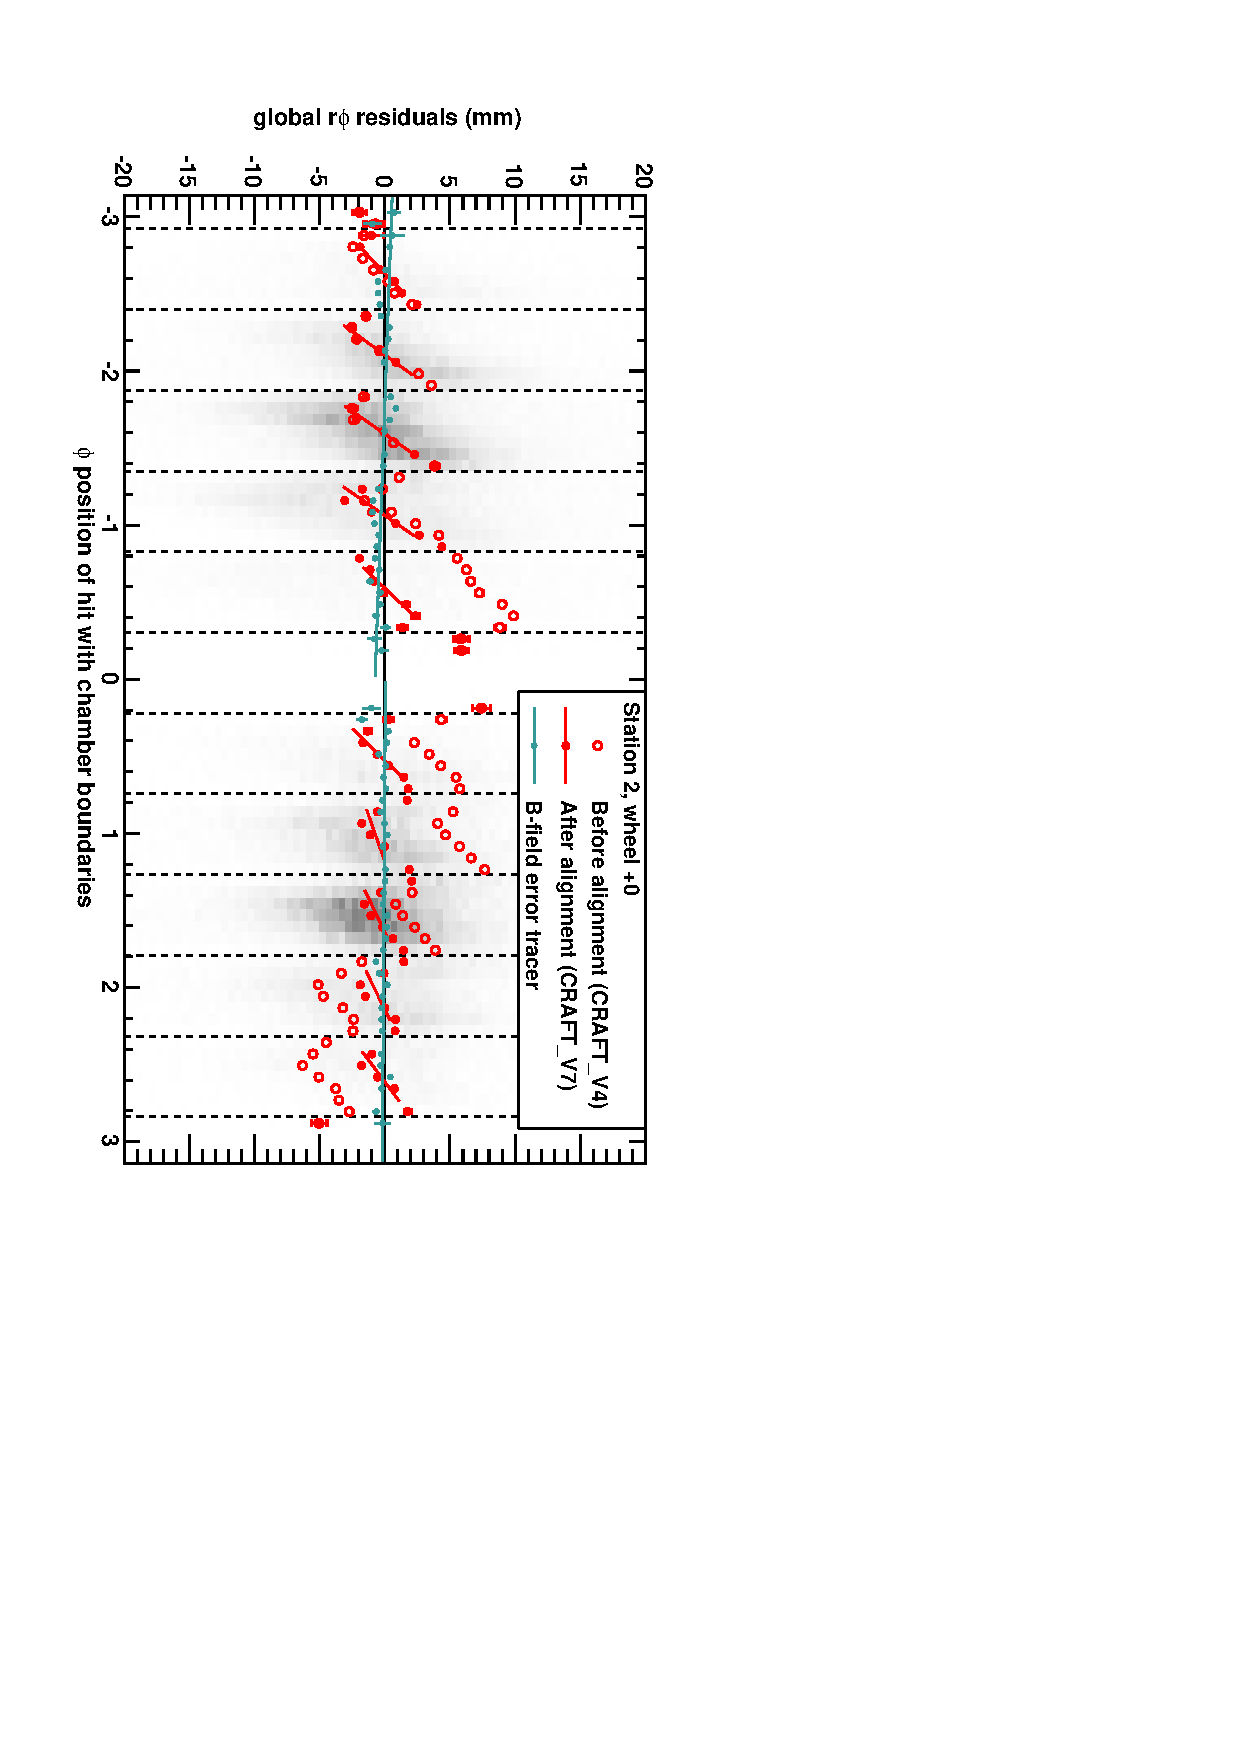
\includegraphics[height=\linewidth, angle=90]{DTrphiVsPhi_st2_whC.pdf}}\only<3>{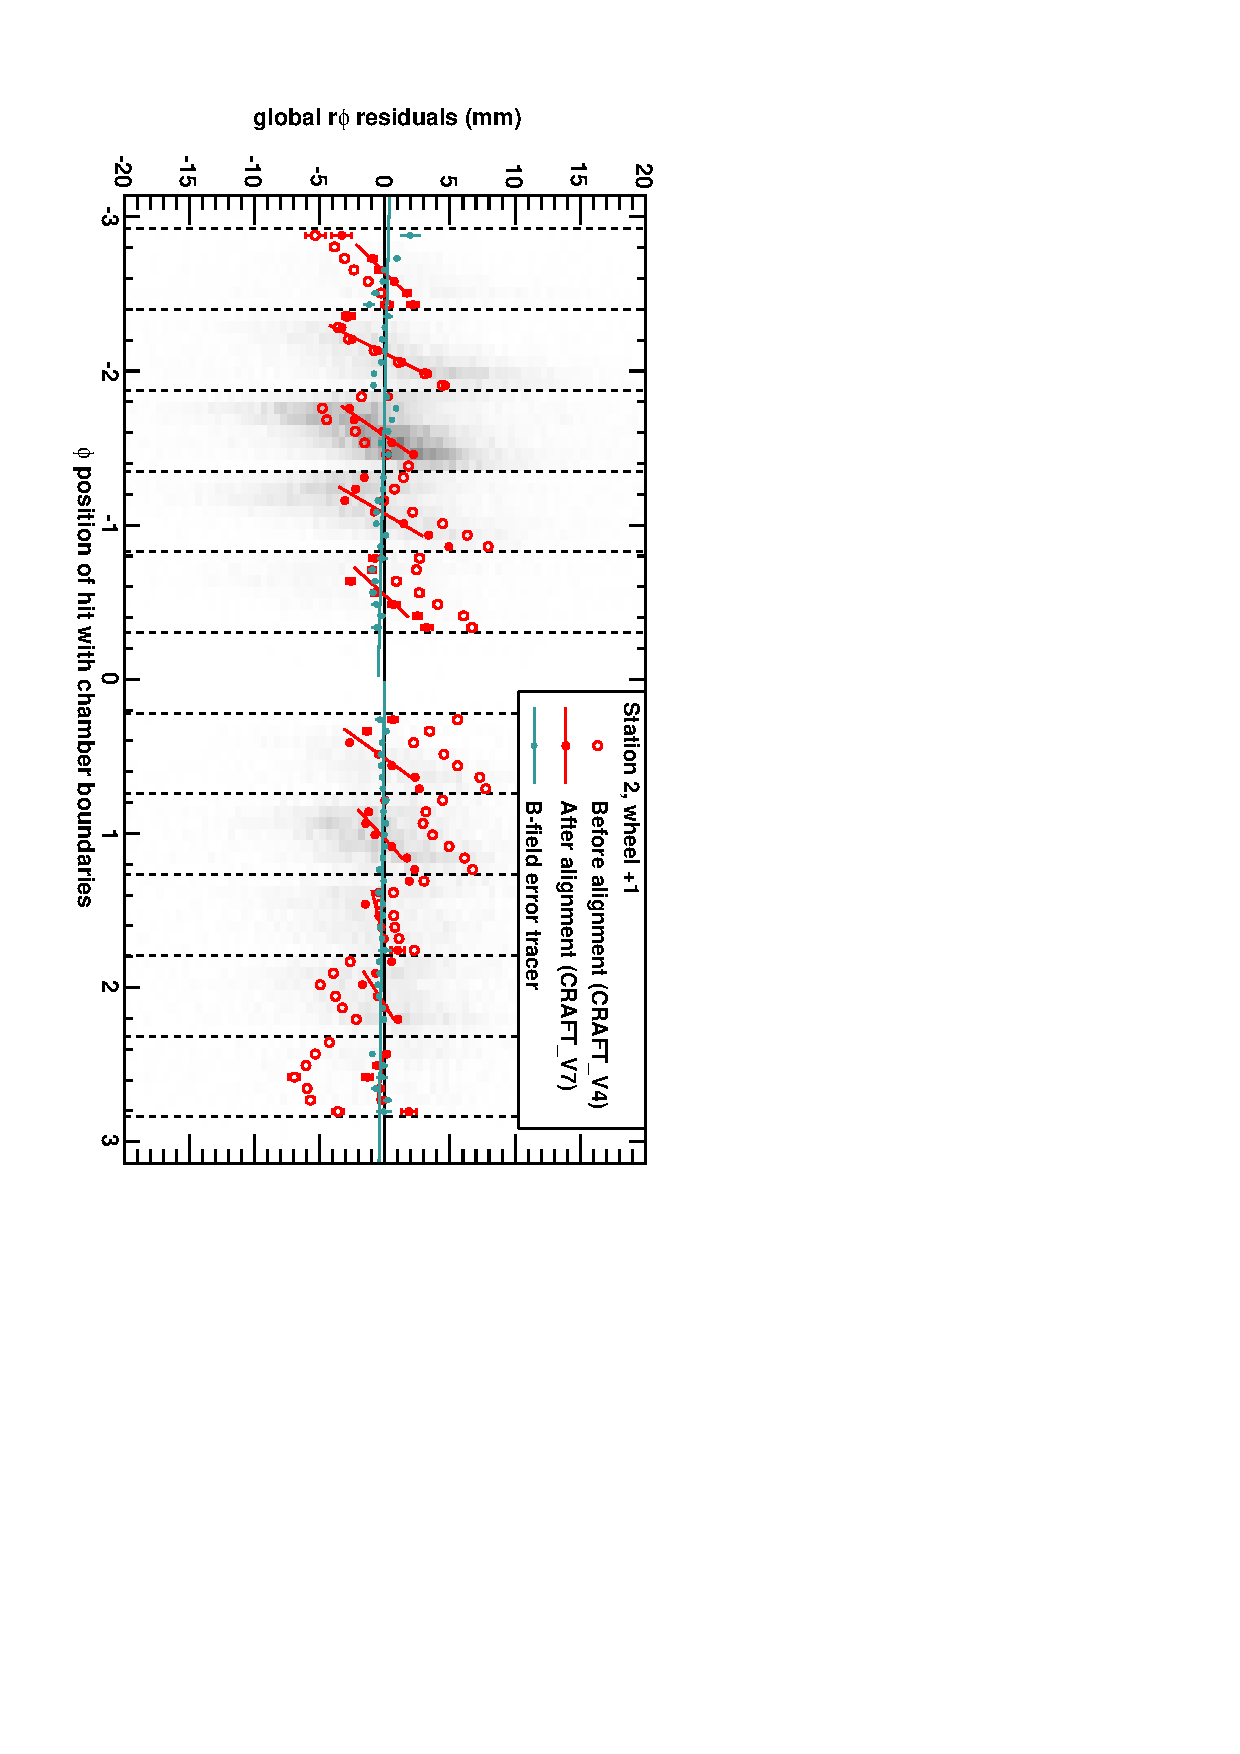
\includegraphics[height=\linewidth, angle=90]{DTrphiVsPhi_st2_whD.pdf}}\only<4>{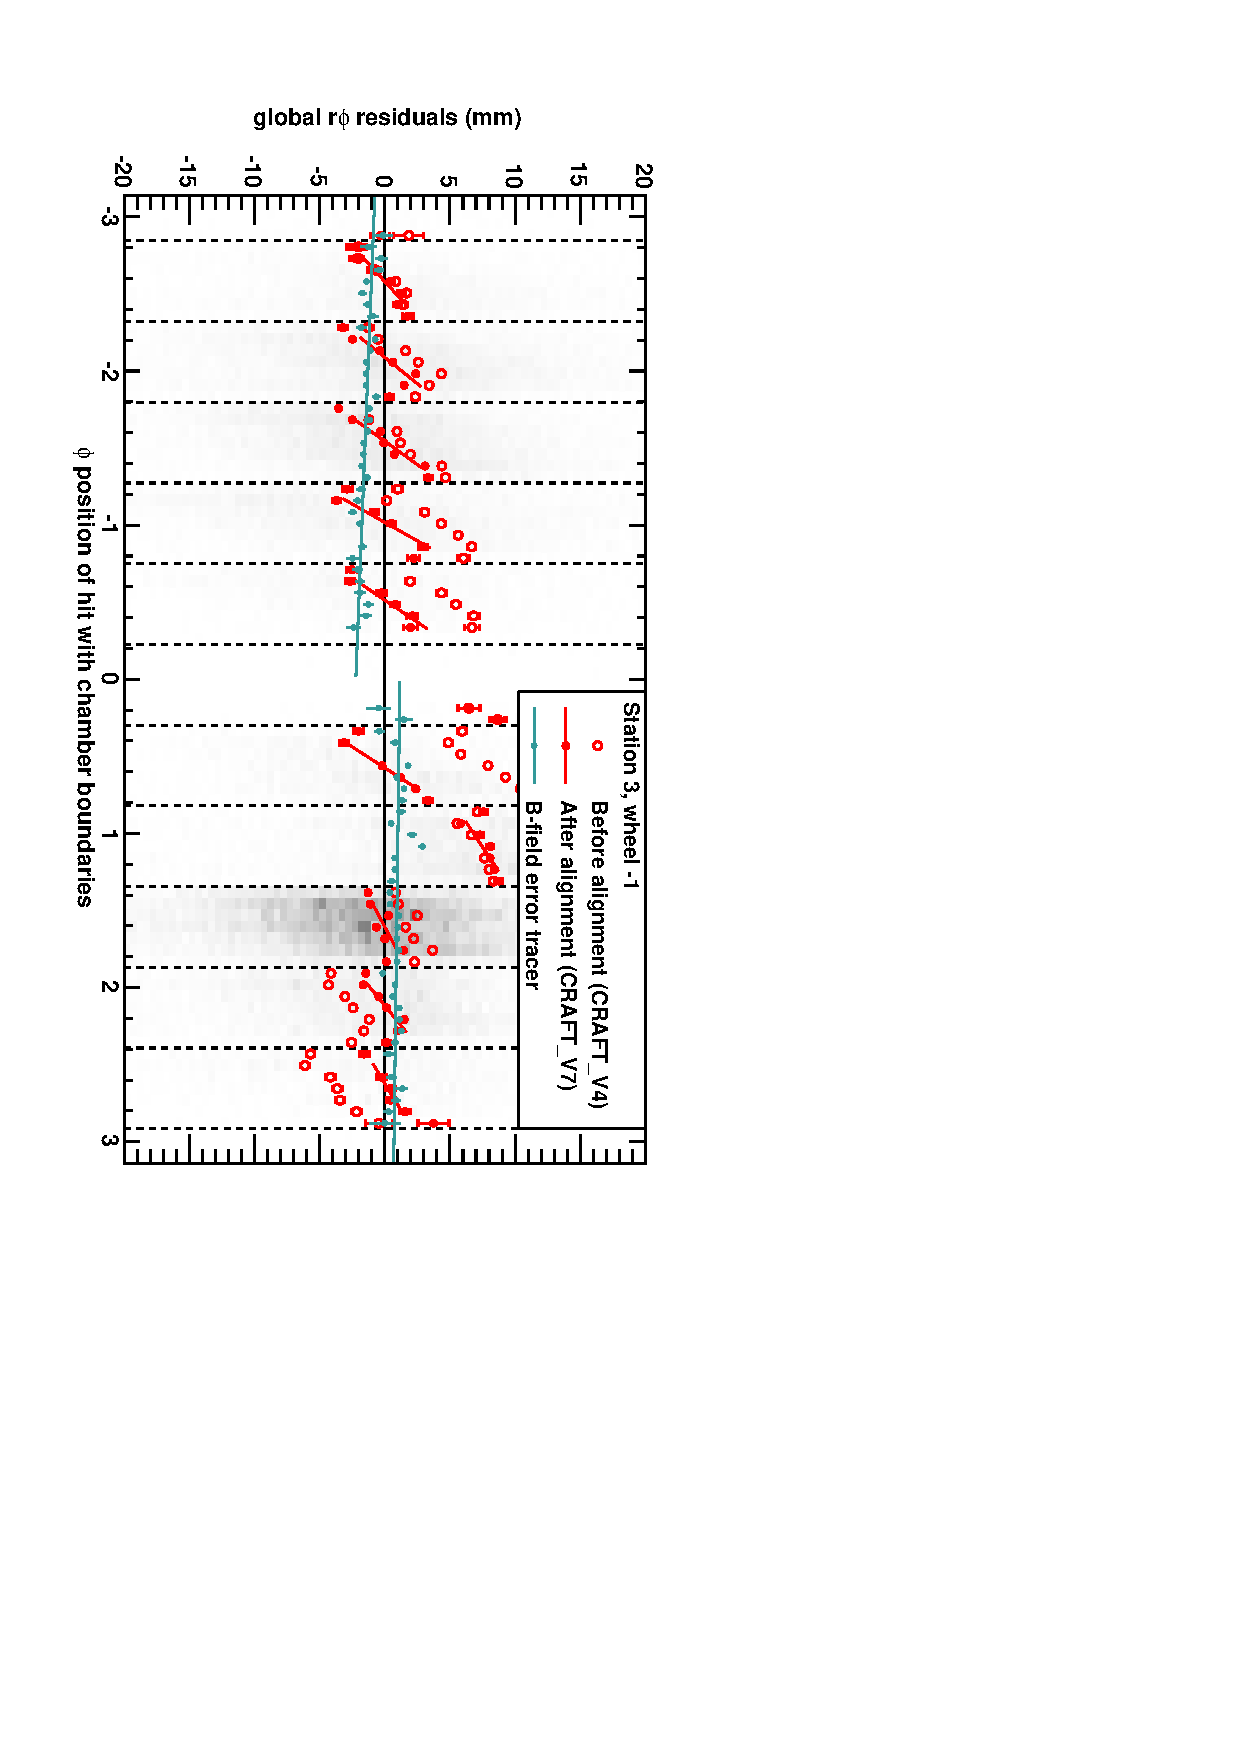
\includegraphics[height=\linewidth, angle=90]{DTrphiVsPhi_st3_whB.pdf}}\only<5>{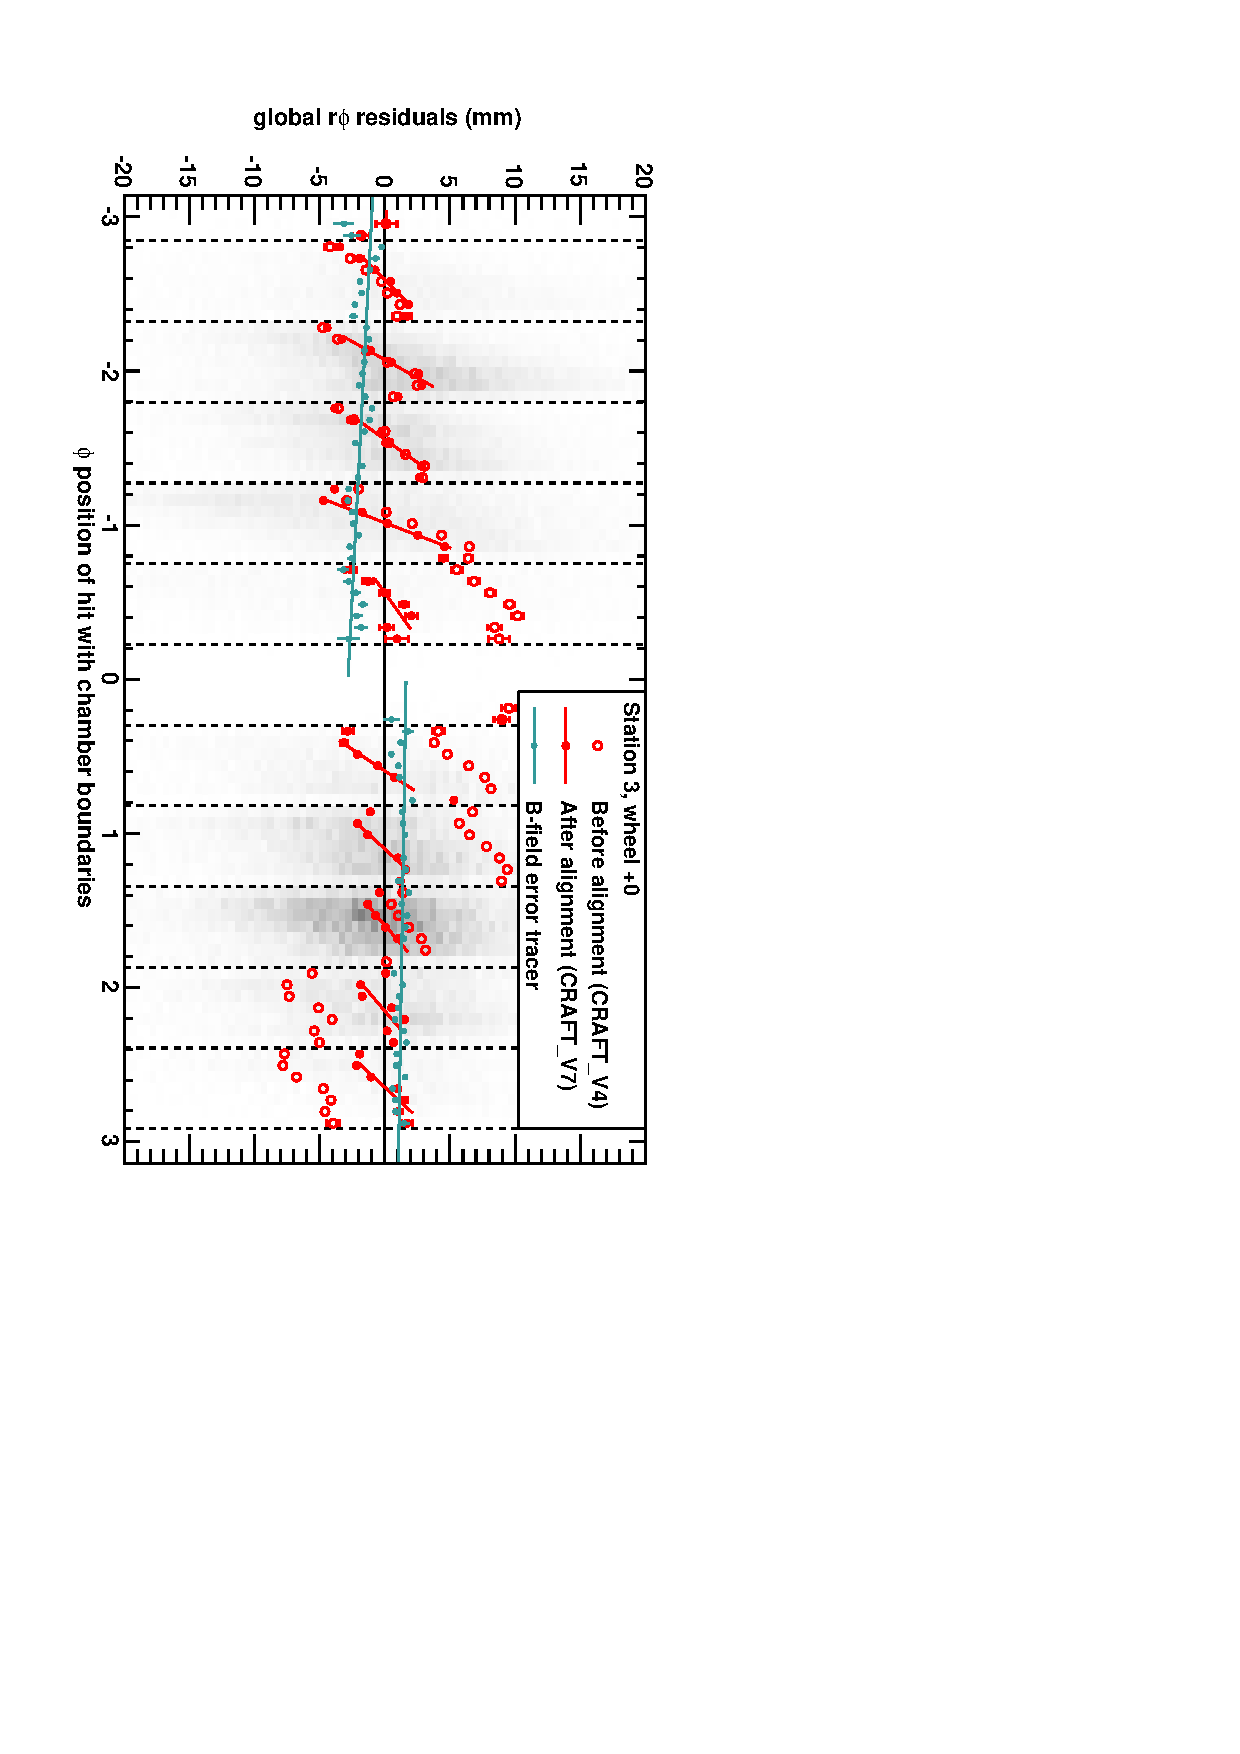
\includegraphics[height=\linewidth, angle=90]{DTrphiVsPhi_st3_whC.pdf}}\only<6>{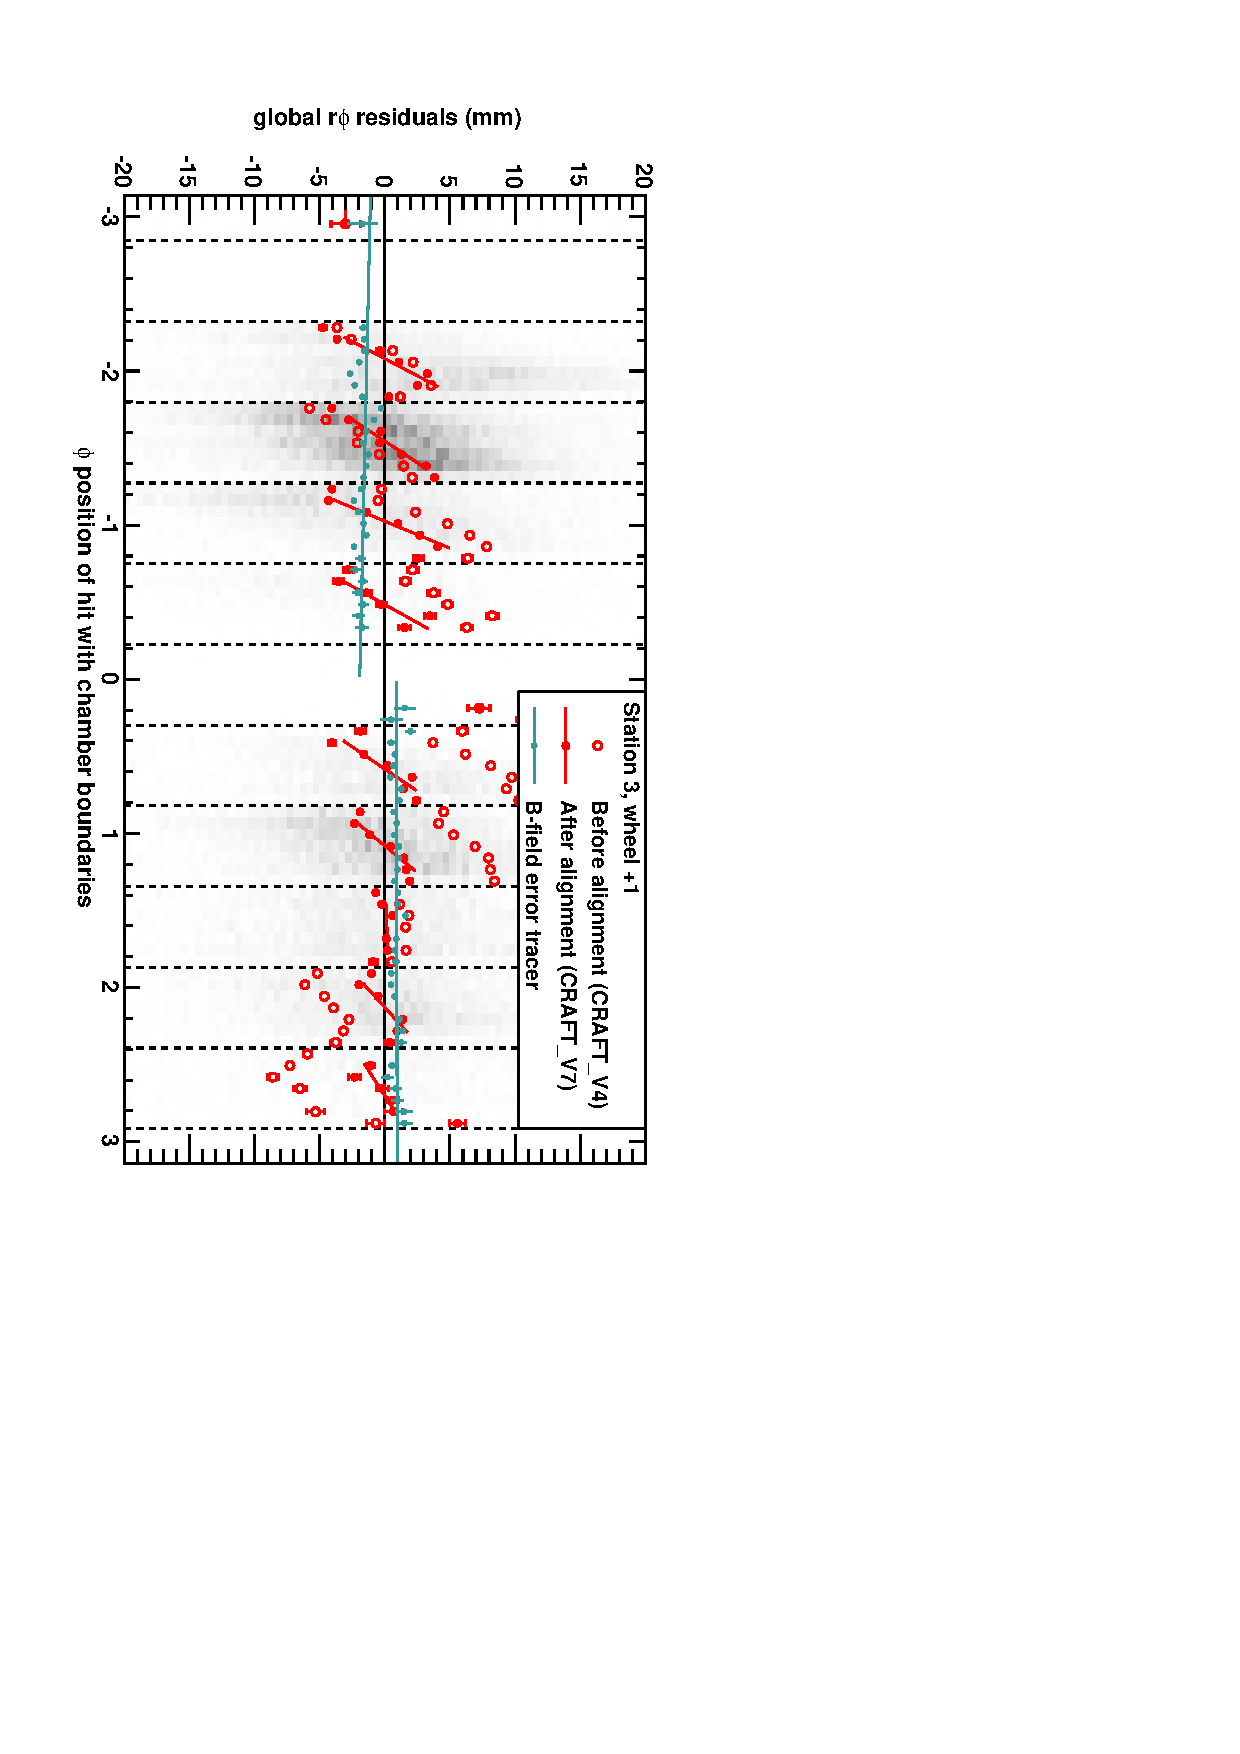
\includegraphics[height=\linewidth, angle=90]{DTrphiVsPhi_st3_whD.pdf}}\only<7>{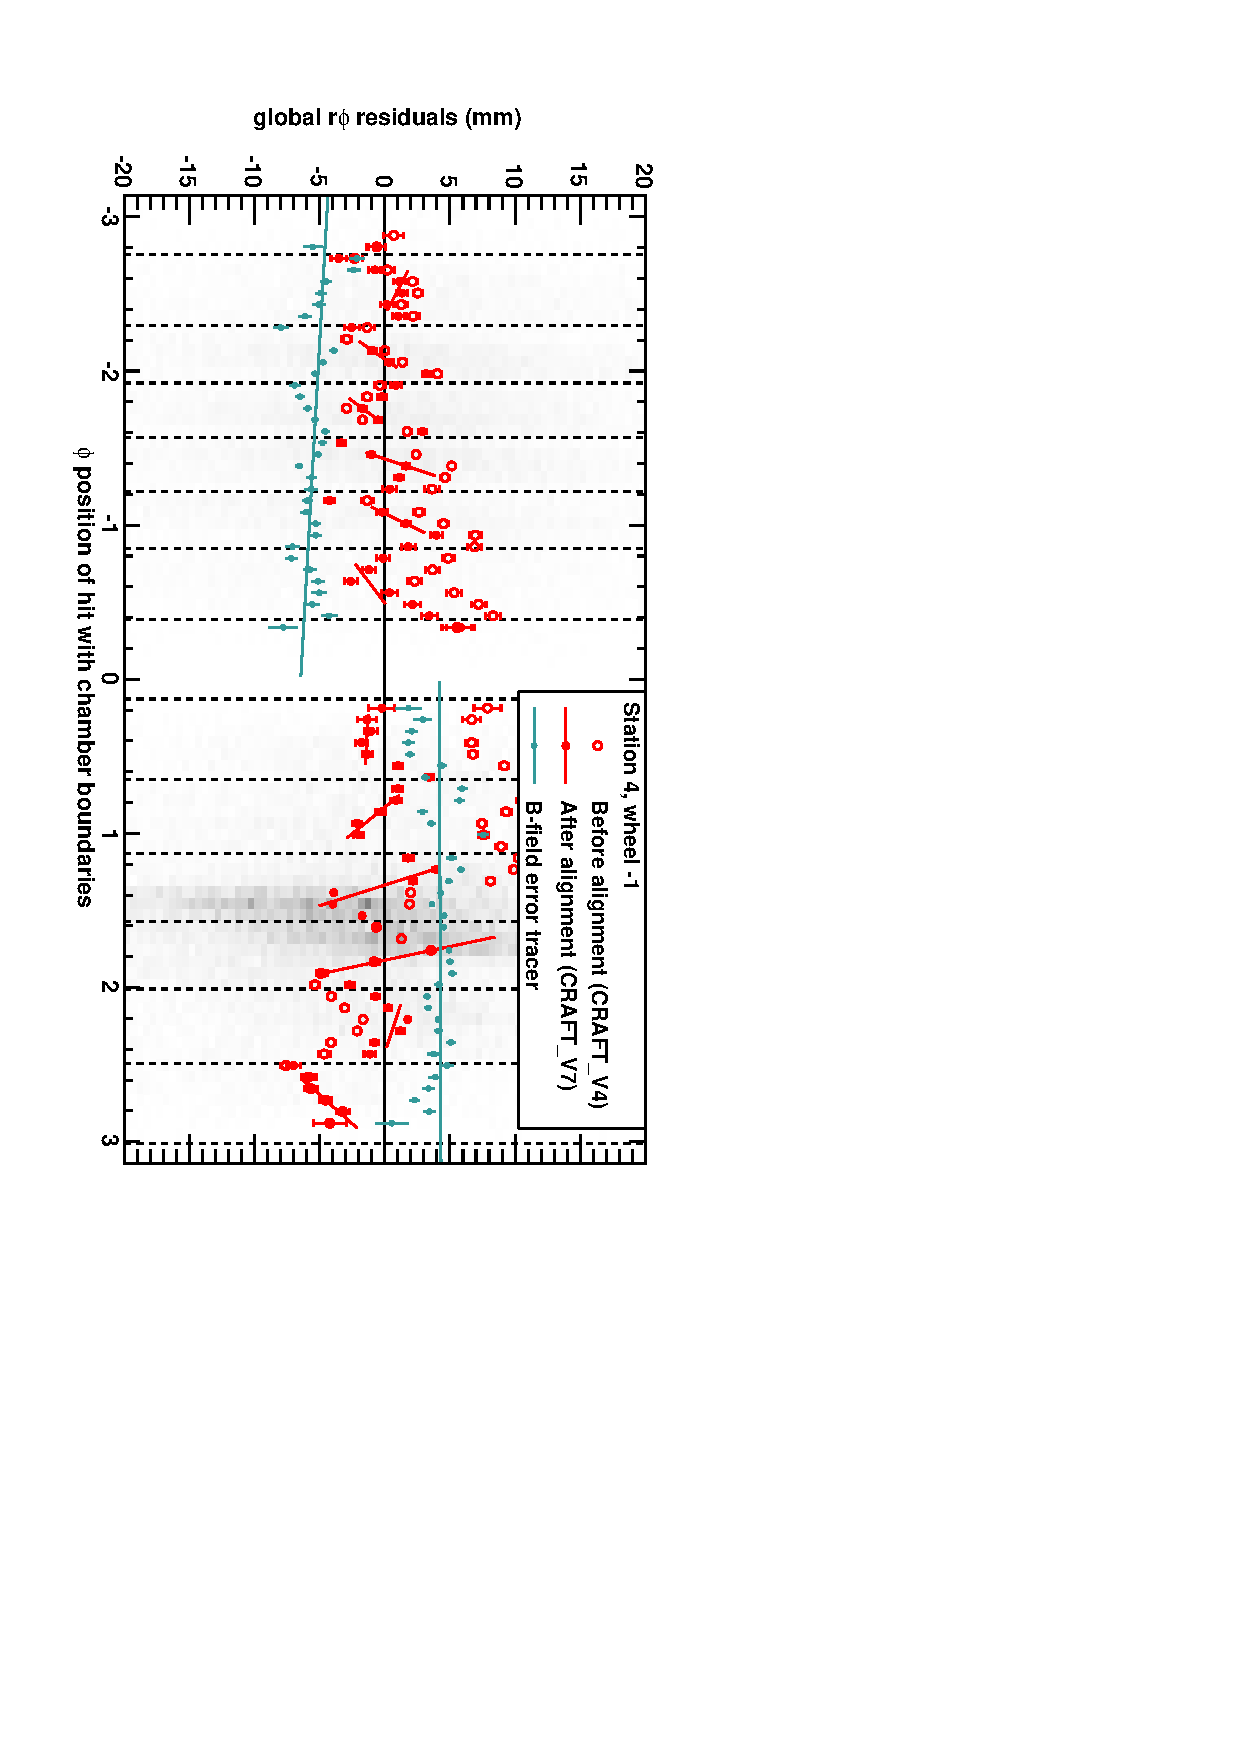
\includegraphics[height=\linewidth, angle=90]{DTrphiVsPhi_st4_whB.pdf}}\only<8>{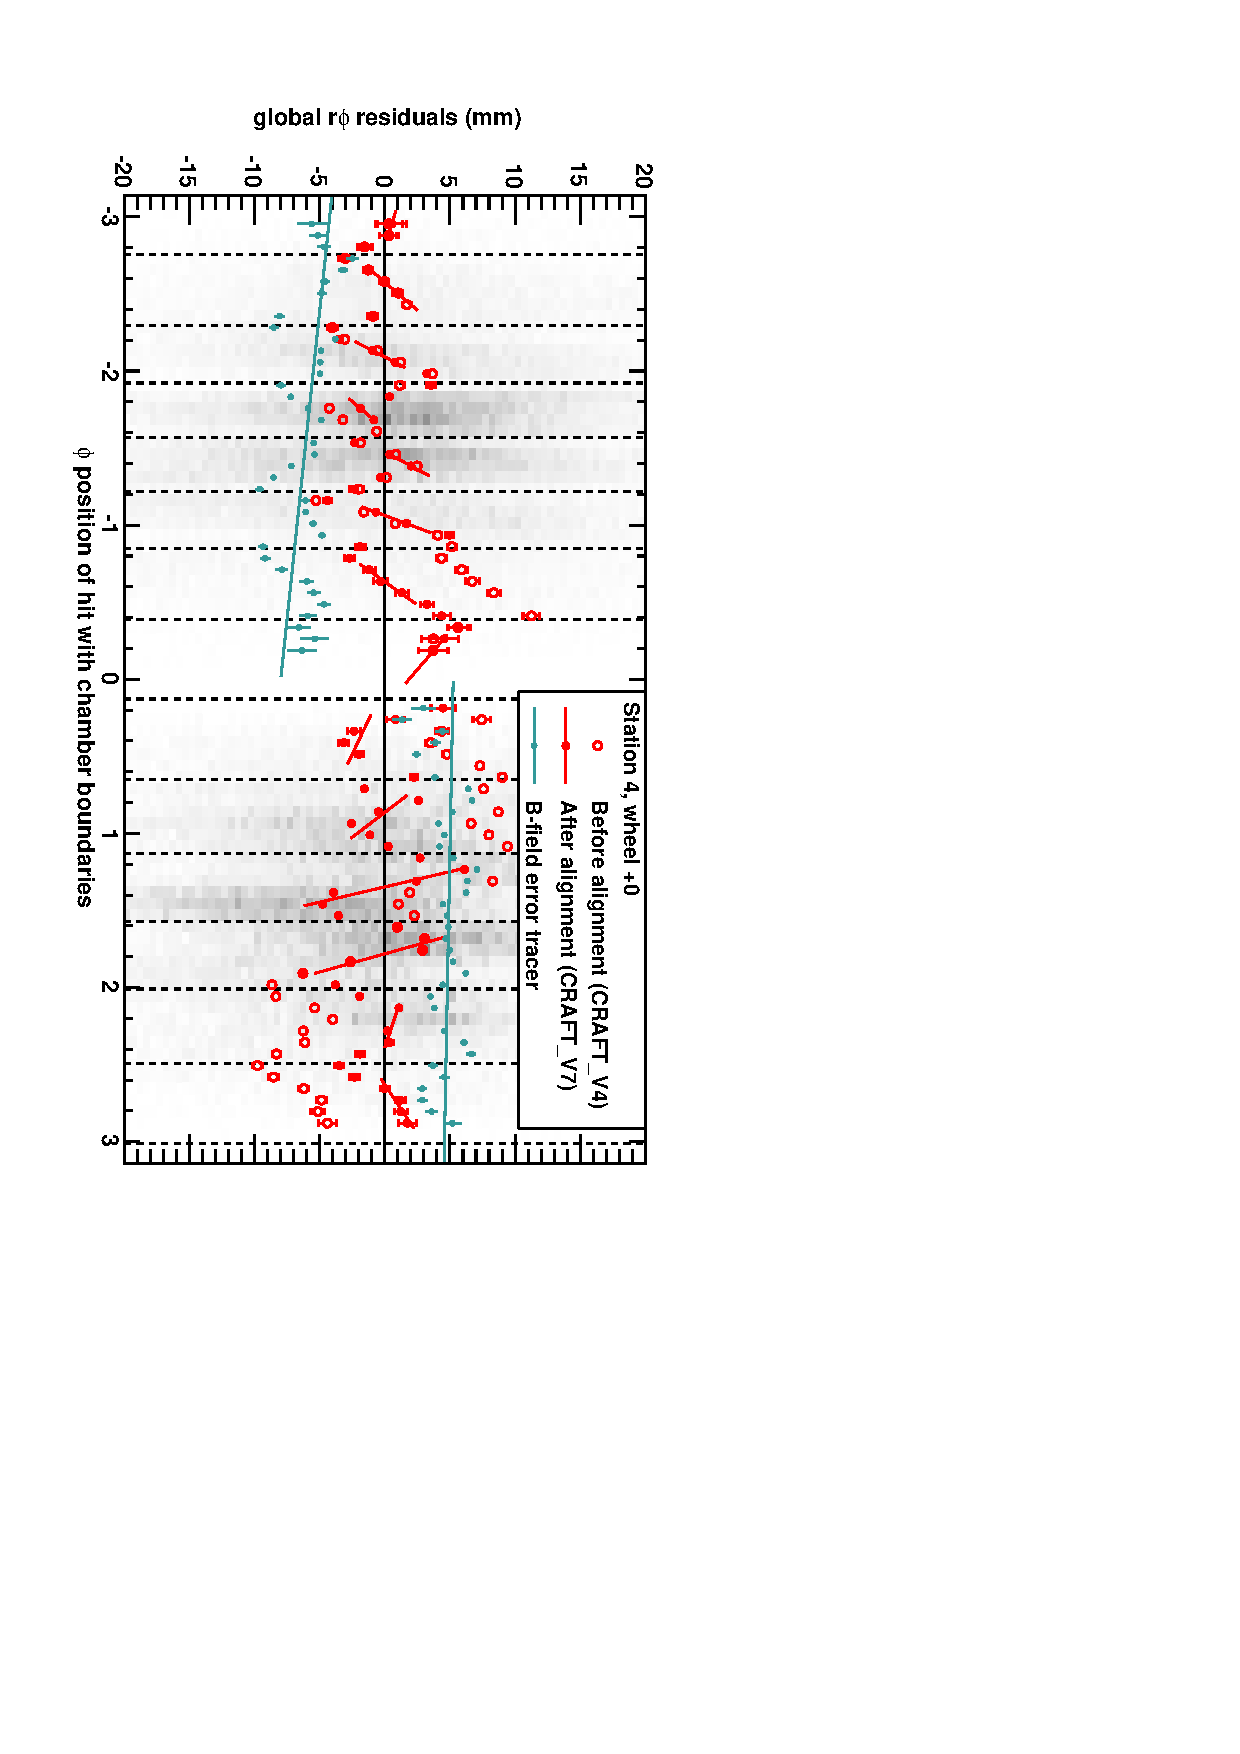
\includegraphics[height=\linewidth, angle=90]{DTrphiVsPhi_st4_whC.pdf}}\only<9>{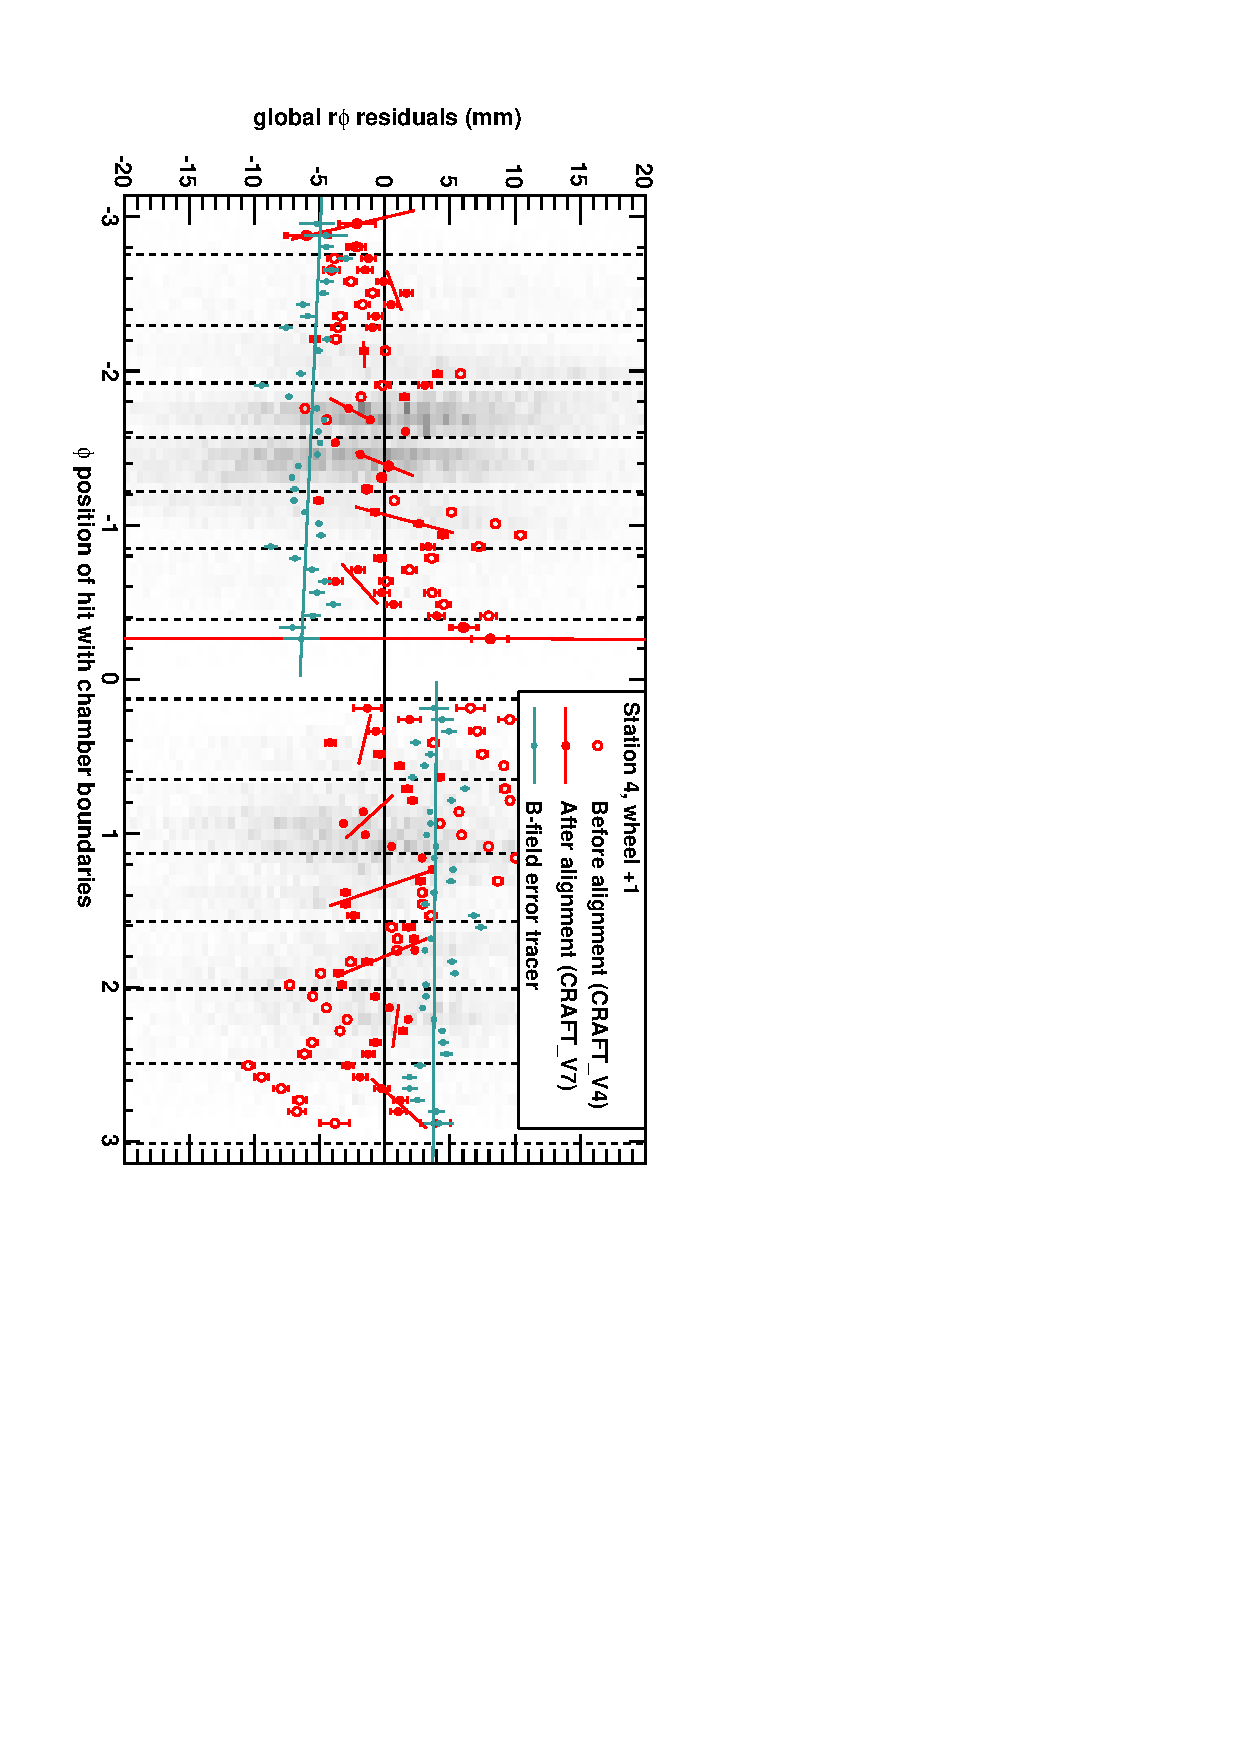
\includegraphics[height=\linewidth, angle=90]{DTrphiVsPhi_st4_whD.pdf}}

\vspace{-0.5 cm}
\begin{itemize}
\item Let's skim through all the plots: \only<1>{station 2, wheel $-$1}\only<2>{station 2, wheel 0}\only<3>{station 2, wheel $+$1}\only<4>{station 3, wheel $-$1}\only<5>{station 3, wheel 0}\only<6>{station 3, wheel $+$1}\only<7>{station 4, wheel $-$1}\only<8>{station 4, wheel 0}\only<9>{station 4, wheel $+$1}
\item<3-> See what I mean about the slopes being roughly the same everywhere?
\item<7-> In station 4, the pattern is less clear because the residuals distributions are much wider and the detector is more finely (and unevenly) divided in $\phi$
\end{itemize}
\end{frame}


\begin{frame}
\frametitle{The $\phi_y$ possibility}

\begin{columns}
\column{0.5\linewidth}
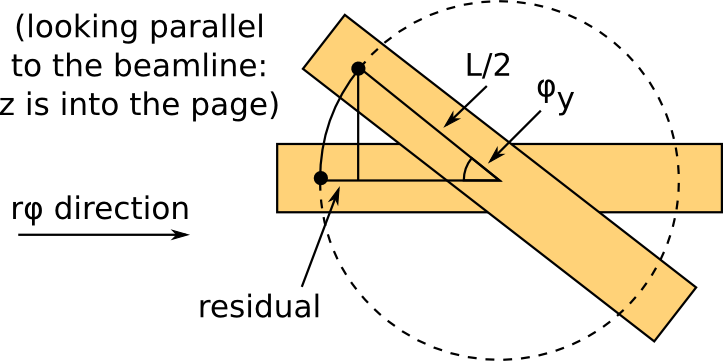
\includegraphics[width=\linewidth]{phiy_explanation.png}

\column{0.5\linewidth}
\begin{itemize}
\item $\phi_y$ rotation can make a chamber appear narrower
\item but it's a second-order effect:
\end{itemize}

\vspace{-0.75 cm}
\begin{eqnarray*}
\mbox{residual} &=& (L/2) \left(1 - \cos\phi_y\right) \\
\mbox{0.25 cm} &\approx& \frac{\mbox{200 cm}}{2} \left(\frac{{\phi_y}^2}{2}\right) \\
\phi_y &\approx& \mbox{70~mrad}
\end{eqnarray*}
\end{columns}

\vfill
\begin{itemize}
\item Could {\it all} the chambers be independently misaligned by about 70~mrad?
\item Same effect observed in IDEAL and CRAFT\_ALL\_V4 constants: it
  would have to be a physical misalignment of real chambers
\item I think we can safely say that this is not what's happening
\begin{itemize}
\item the magnitude is too big, and
\item the pattern is too regular
\end{itemize}
\end{itemize}
\end{frame}

\begin{frame}
\frametitle{The $\Delta R$ possibility}

\begin{columns}
\column{0.7\linewidth}
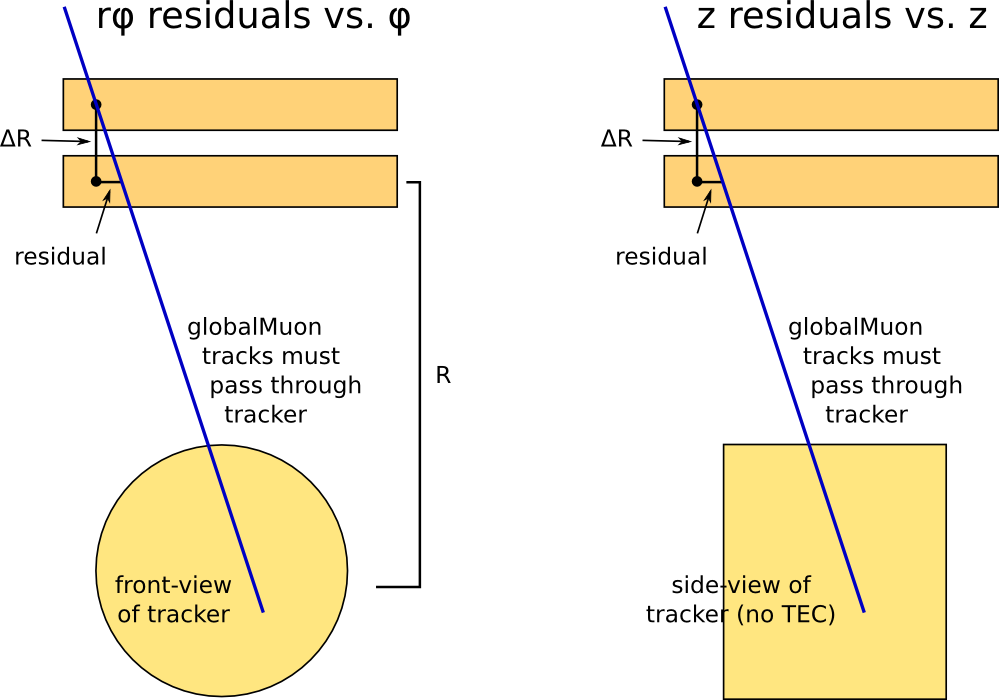
\includegraphics[width=\linewidth]{z_explanation.png}

\column{0.3\linewidth}
\begin{itemize}
\item A track sample constrained to pass through the tracker can introduce effects of this sort

\vspace{0.2 cm}
\mbox{\hspace{-1 cm}$\displaystyle \Delta R = \frac{R}{(L/2)} \left(\mbox{residual}\right)$\hspace{-1 cm}}

\vspace{0.1 cm}
\item But it has to appear in both types of residuals
\end{itemize}
\end{columns}
\end{frame}

\begin{frame}
\frametitle{Trial $\Delta R$ alignment (1/2)}

\begin{itemize}
\item To see if this is plausible, I expanded the radius of all DT stations by 15~mm in a private test
\begin{itemize}
\item seems to cancel the $r\phi$ residual vs.\ $\phi$ trend in the $-\pi < \phi < 0$ range, but overshoot slightly in the $0 < \phi < +\pi$ range
\end{itemize}
\end{itemize}

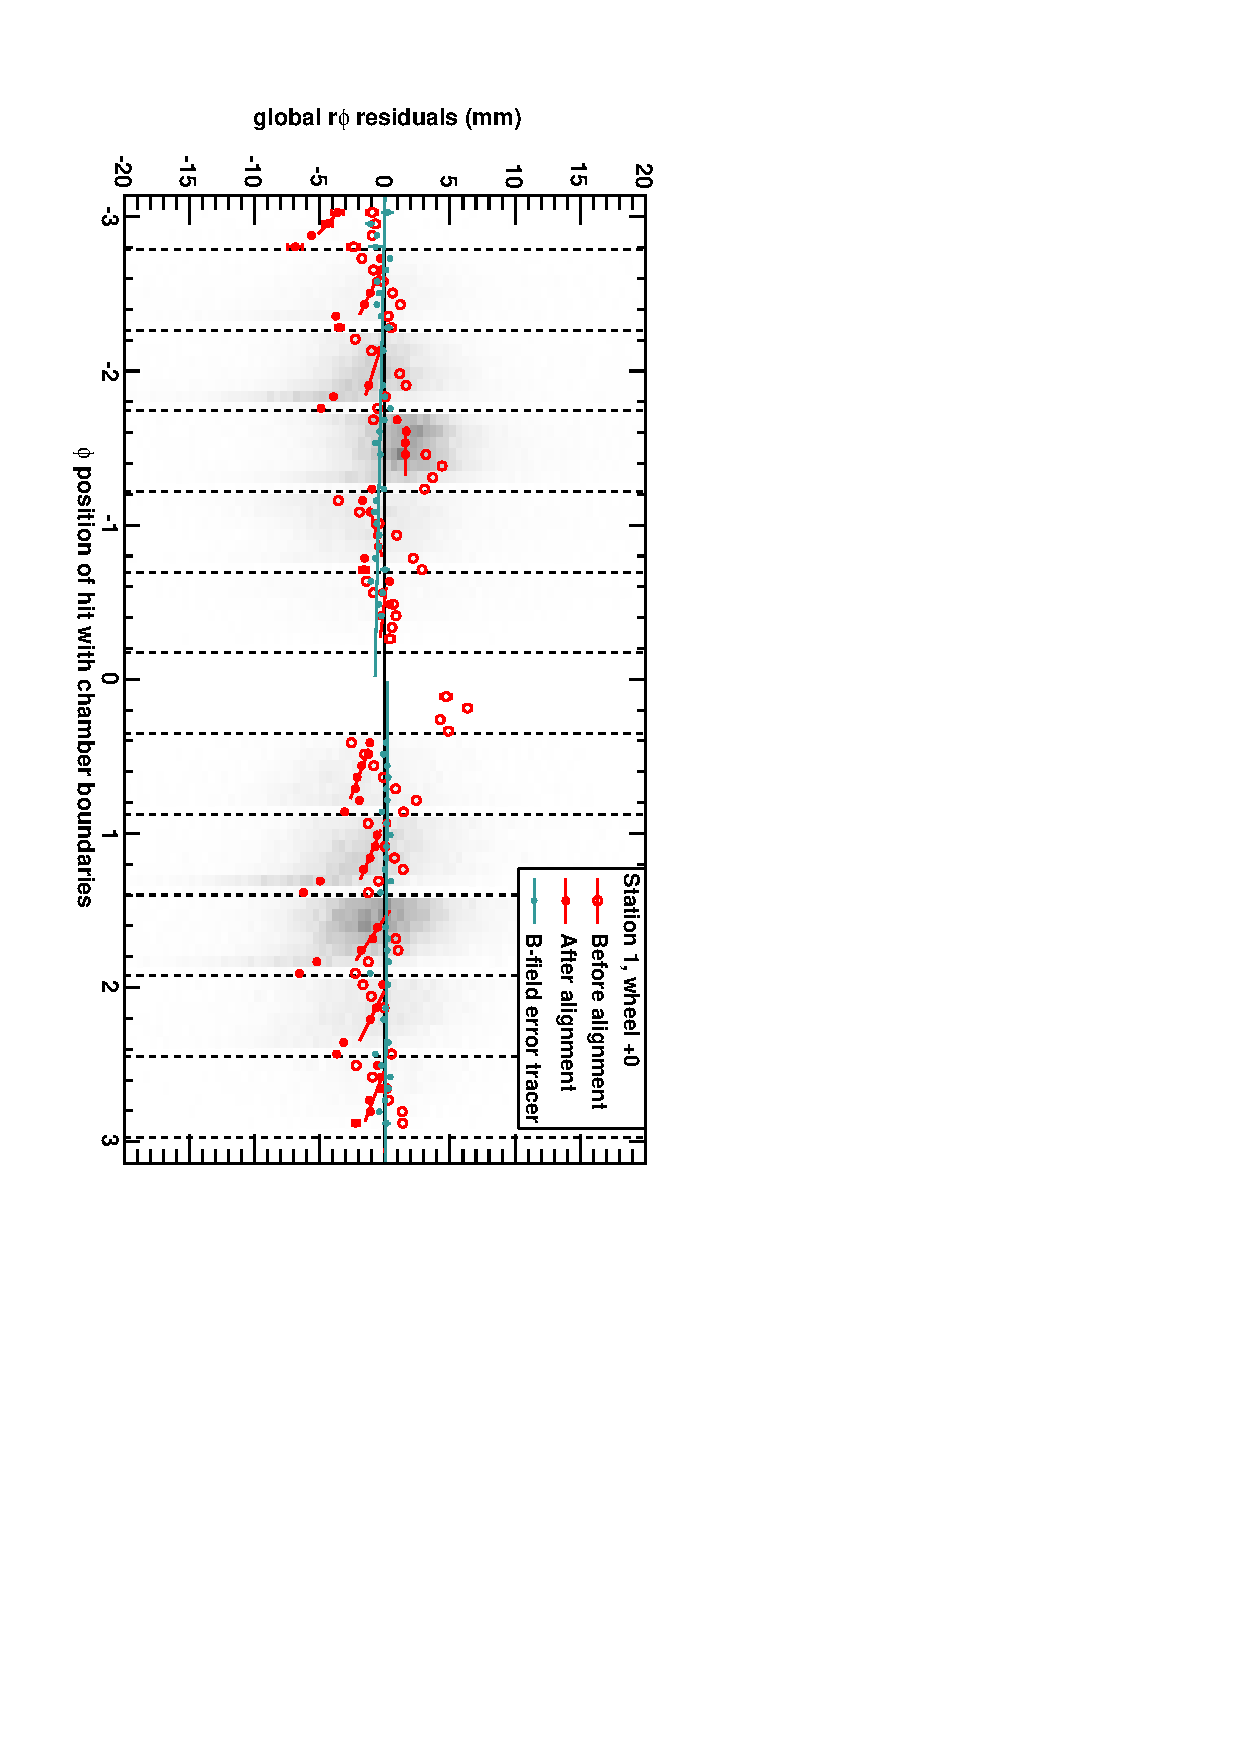
\includegraphics[height=\linewidth, angle=90]{DTrphiVsPhi_st1_whC_out15mm.pdf}
\end{frame}

\begin{frame}
\frametitle{Trial $\Delta R$ alignment (2/2)}

\begin{itemize}
\item However, look what happens to the $z$ residual vs.\ $z$: clearly both types of residuals can't be satisfied!
\item The open circles are the case of no $\Delta R$ shift
\end{itemize}

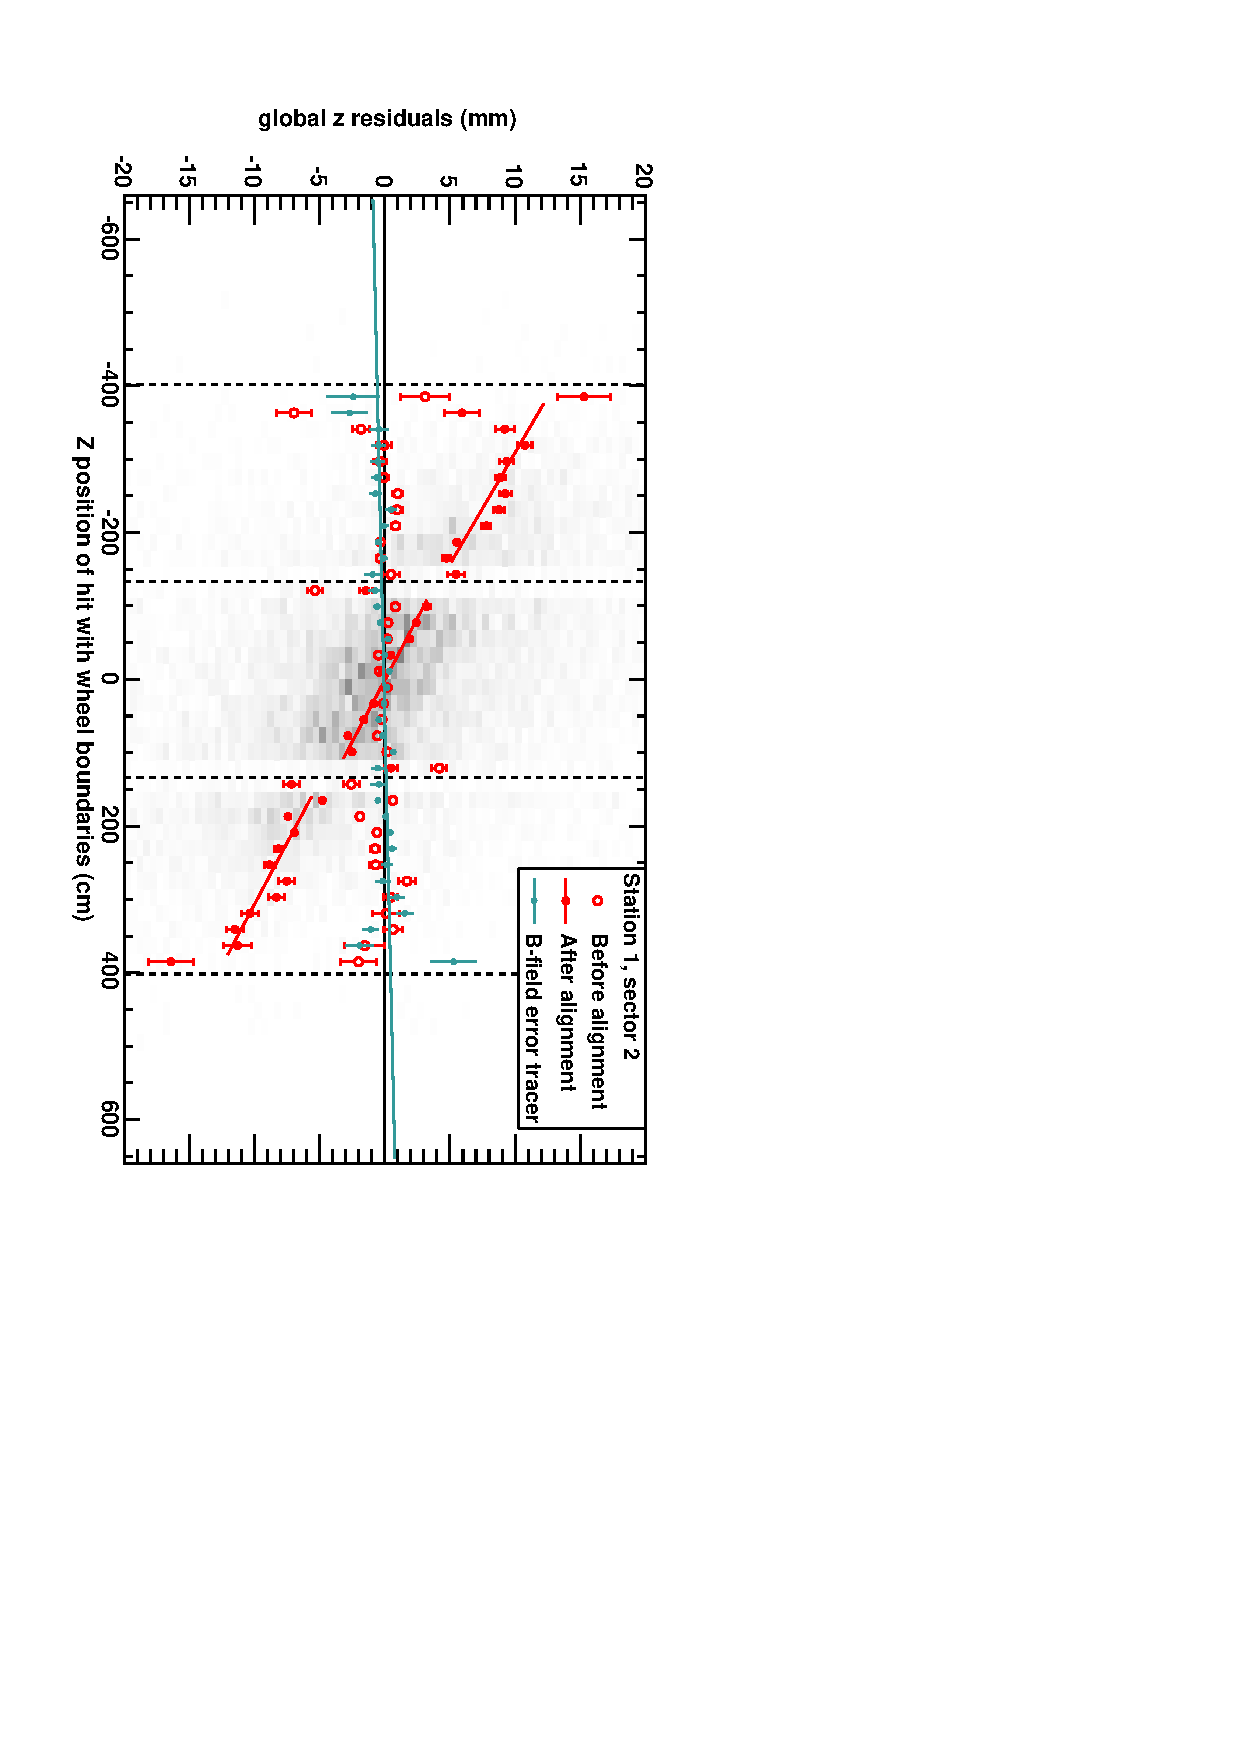
\includegraphics[height=\linewidth, angle=90]{DTzVsZ_st1_sr02_out15mm.pdf}
\end{frame}

\begin{frame}
\frametitle{So, what could it be?}

\begin{itemize}
\item Process of elimination for all rigid body degrees of freedom

\begin{itemize}
\item \sout{$\phi_y$: implausible}
\item \sout{$\Delta R$ (a $\Delta R$ translation): can't reconcile both $r\phi$ and $z$ residuals}
\item local $x$, $y$ translations: can't introduce any linear trends in residuals, only offsets
\item $\phi_z$ rotation: introduces a linear trend in $r\phi$
  residuals vs.\ $z$ and $z$ residuals vs.\ $\phi$, but not what we're
  looking for
\item $\phi_x$ rotation: also would have to be implausibly large, and only affects $z$ residuals (the opposite of what we're looking for)
\end{itemize}

\item Non-rigid degree of freedom \hfill 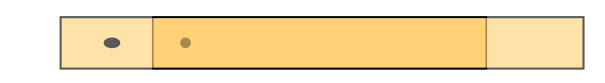
\includegraphics[width=0.35\linewidth]{stretch_explanation.png}

\begin{itemize}
\item {\it some kind} of stretching would easily explain it
\item an error in the geometry description, duplicated by CMSSW, would
  account for its regularity (with outliers due to individual
  $\Delta R$ misalignments)
\end{itemize}
\end{itemize}
\end{frame}

\begin{frame}
\frametitle{Analogy with CSC case}
\begin{itemize}
\item Last year, track-based alignment found 0.8~mm error in CSC widths
\item For the same reasons, chamber stretching was degenerate with increasing the distance from the beamline
\item Degeneracy was resolved with photogrammetry of alignment pins
\begin{itemize}
\item track-based procedure reproduced $r\phi$ positions of alignment pins with 270~$\mu$m accuracy
\item $R$ positions of pins were therefore directly comparable, and constrained distance from the beamline
\end{itemize}
\item CSC geometry experts investigated and quickly found a 10~$\mu$m strip pitch
  angle error, which, compounded over 80~strips, changed the width by
  0.8~mm, explaining the observation with tracks
\item Error was in an XML file, not the database, and originated in miscommunication (design values rather than measured)
\item DTs have an advantage over CSCs in that they precisely measure
  $z$ residuals in addition to $r\phi$ residuals, so we can already
  break degeneracy between $\Delta R$ and stretching
\item In the CSC case, we got the sign wrong, but not magnitude
\end{itemize}
\end{frame}

\begin{frame}
\frametitle{What kinds of distortions?}
\begin{itemize}\setlength{\itemsep}{0.25 cm}
\item A literally stretched chamber: e.g.\ small correction in drift
  tube diameter, compounded across the chamber \mbox{(exact analogy with CSC)\hspace{-1 cm}}
\item An effective 70~mrad rotation built into the chamber: angled layer planes
\item A large $\Delta R$ error in superlayer positions, different for each superlayer
\begin{itemize}
\item not what anyone would call ``stretching,'' so I should be careful to not use that terminology for this case
\item we concluded non-rigid body distortion due to incompatibility between $r\phi$ residuals vs.\ $\phi$ and $z$ residuals vs.\ $z$; perhaps the incompatibility is built into the chamber
\item unfortunately, the scale would have to be $\mathcal{O}(\mbox{10~mm})$, which I think is ruled out
\end{itemize}
\item \ldots more?
\end{itemize}
\end{frame}

\begin{frame}
\frametitle{Non-geometric explanations?}
\begin{itemize}

\item A timing effect?
\begin{itemize}
\item I don't think any drift time effect could explain it, since we
  don't have the spatial resolution to see the difference between the
  left and right sides of each wire
\end{itemize}
\item $\vec{B}$-field on electron drift?  No, the
  magnitude of the effect we're seeing is about the same in stations 1, 2,
  and 3
\item We should continue considering possibilities that it's a tracking effect
\begin{itemize}
\item constraint: it {\it must} be an effect in the chamber, not the track source, since it knows about chamber boundaries
\item \sout{could the chamber material act like a lens?  Difference in speed of muons in material causes refraction?}  (such an effect would need to be much larger in the iron)
\end{itemize}
\item I should apply this machinery to layer-by-layer residuals, see if there's a revealing pattern (multiplying number of plots by 6)
\end{itemize}
\end{frame}

\begin{frame}
\frametitle{$\Delta R$s are misaligned, too}

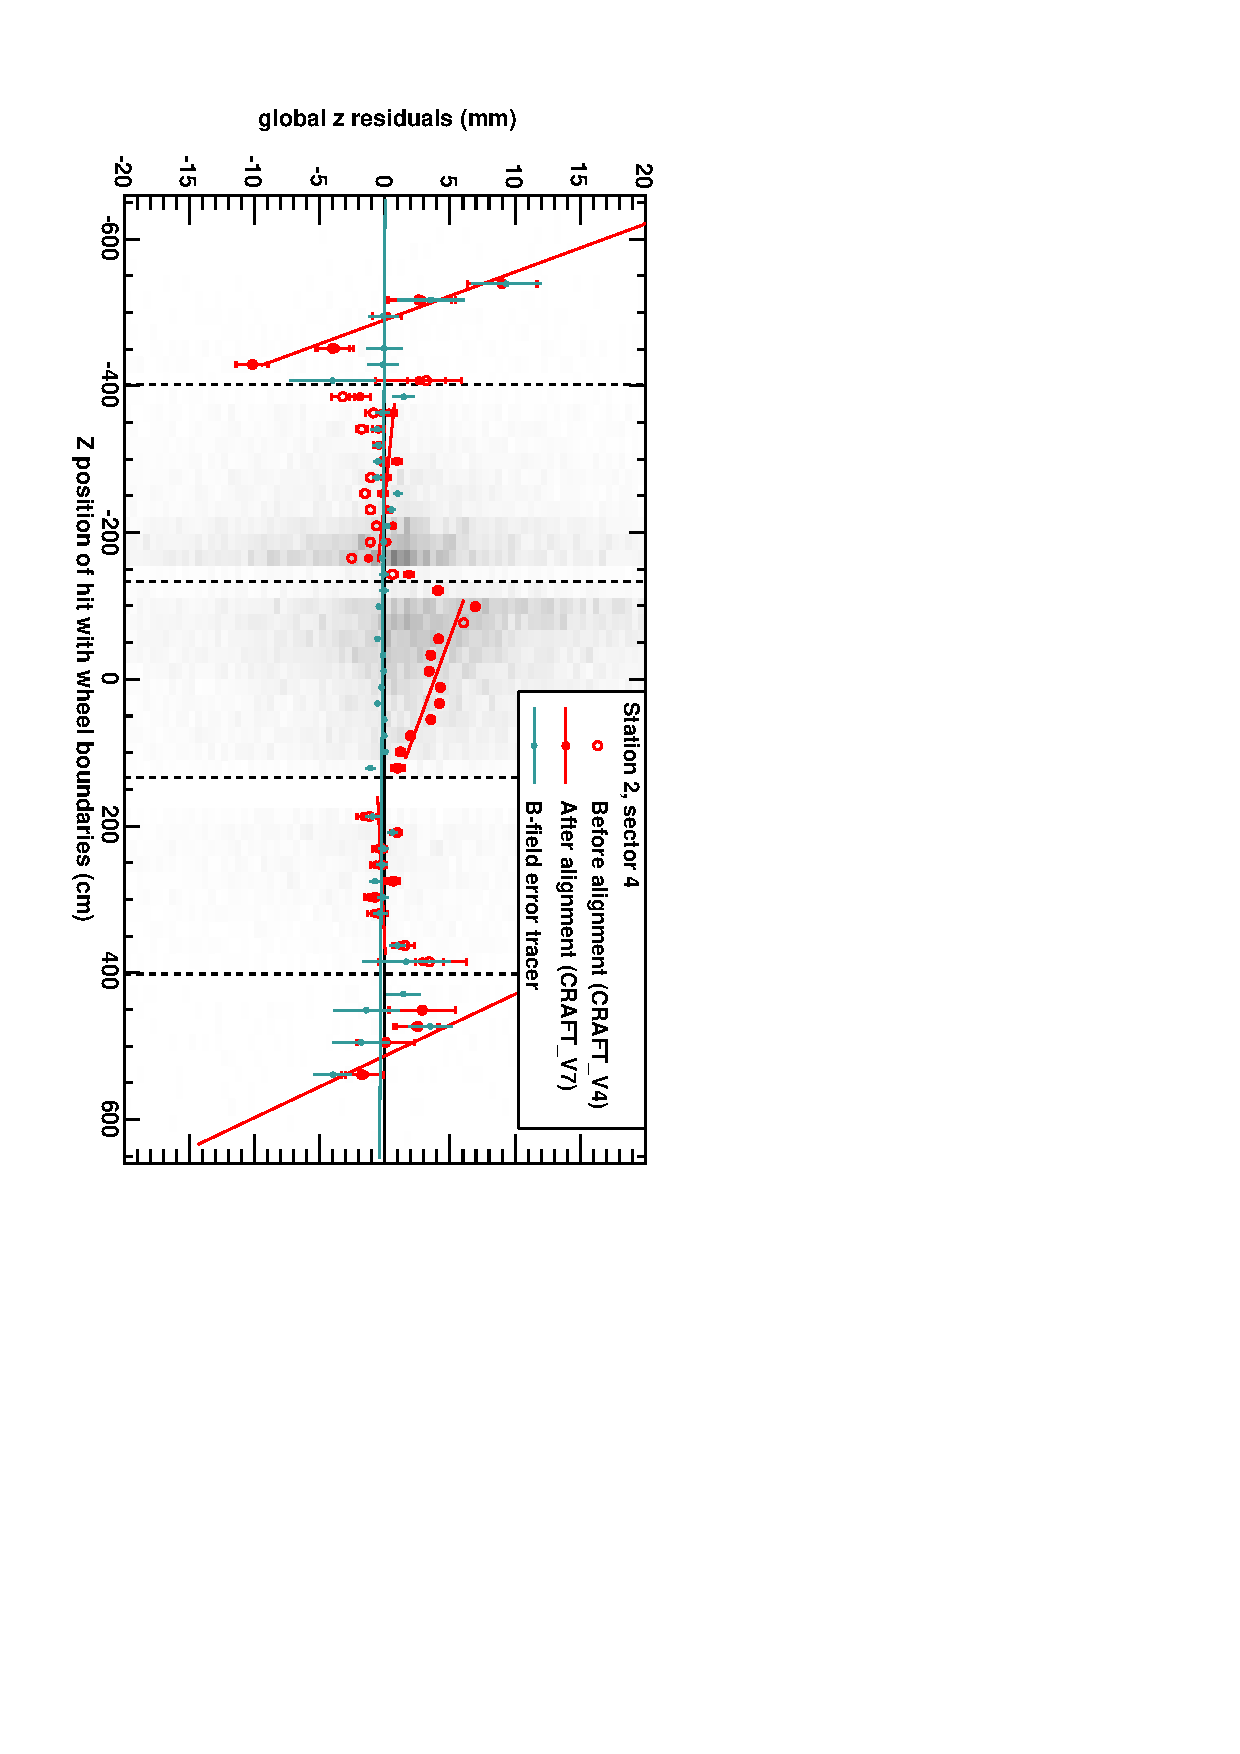
\includegraphics[height=\linewidth, angle=90]{DTzVsZ_st2_sr04.pdf}

\begin{itemize}
\item While the $r\phi$ residuals vs.\ $\phi$ slopes and $z$ residuals vs.\ $z$ slopes can't both be resolved by a single $\Delta R$ translation, some chambers seem to be additionally misaligned in that direction
\item After the ``stretch'' issue is resolved, we'll know how to correct these misalignments
\end{itemize}
\end{frame}

\begin{frame}
\frametitle{Summary}
\begin{itemize}
\item $r\phi$ residuals show clear and clearly-regular trends vs.\ $\phi$
\item The simple possibility--- a rigid-body translation or
  rotation--- can't explain it on the chamber level
\begin{itemize}
\item demonstrated with explicit tests
\end{itemize}

\item DT stretching would be the next natural possibility
\begin{itemize}
\item geometry experts investigating\ldots
\end{itemize}

\item Non-geometric explanations are welcome, but highly constrained

\item Though the regular pattern can't conform to a universal radial correction,
  some radial positions will need to be corrected afterward
\end{itemize}
\label{numpages}
\end{frame}

\end{document}
